\documentclass[12pt, a4paper]{article}
%\documentclass[AEJ, reviewmode]{AEA}
\usepackage{authblk}
\usepackage{float}
\usepackage{tabls}
\usepackage{graphicx}
\usepackage{parskip}
\usepackage{amsmath}
\usepackage{setspace} %for setting line spacing

\usepackage{lscape} %for using landscape 
%\usepackage[sectionbib]{natbib} %for more flexible referencing
%\usepackage{chapterbib} % For a separate bibliography for each section
%\usepackage[natbib=true,backend=bibtex,style=authoryear]{biblatex}
\usepackage[comma]{natbib} %for more flexible referencing

\usepackage{url} %for website addresses
\usepackage{dcolumn} %for decimal point alignment
\usepackage{booktabs} %for professionaly looking tables
\usepackage{tabularx} % for creating tables
\usepackage{multirow} % columns spanning multiple rows
%\usepackage{geometry} % for setting margins
\usepackage[in]{fullpage} % for smaller margins
%\usepackage[pdftex,bookmarks=true]{hyperref} % for creating links within the document (to references, tables, equations) or to websites and creating bookmarks
\usepackage[multiple, stable, bottom]{footmisc}% for multiple footnotes at the same place
\usepackage{appendix} % to create separate appendices for each section
\usepackage{changepage}
\usepackage{xcolor}
\usepackage{longtable,pdflscape,booktabs} % to extend tables over multiple pages
\usepackage{enumerate}

\usepackage[textsize=tiny]{todonotes} % todos and comments

\urlstyle{same}
%\floatstyle{plaintop} 
%\restylefloat{table}
%\floatstyle{plain} 
%\restylefloat{figure}
\newcommand{\floatintro}[1]{\vspace*{0.1in} {\footnotesize #1} \vspace*{0.1in}}
\newcolumntype{d}[1]{D{.}{\cdot}{#1}}
\newcolumntype{.}{D{.}{.}{-1}}
\newcolumntype{,}{D{,}{,}{2}}
{\def\sym#1{\ifmmode^{#1}\else\(^{#1}\)\fi}
\raggedbottom % To prevent white spaces between paragraphs

\widowpenalty=10000
\clubpenalty=10000
%\hyphenpenalty=1000
\setcounter{page}{1}
%\geometry{left=1.5in,right=1.5in,top=1.5in,bottom=1.5in}


\title{THE ECONOMIC EFFECT OF GAINING A NEW QUALIFICATION IN LATER LIFE\thanks{\scriptsize{Corresponding author: Anna Zhu, RMIT University. Email: anna.zhu@rmit.edu.au. \newline \newline We thank Tim Robinson, Hayley Fisher, Bruce Bradbury and numerous seminar and conference participants for helpful comments. The authors would like to thank Tessa Loriggio, Prabath Abeysekara, and Yin-King Fok for their excellent research assistance. \newline \newline Zhu acknowledges the support of the Australian Research Council Linkage Project (LP170100472). This paper uses unit record data from the Household, Income and Labour Dynamics in Australia (HILDA) Survey. The HILDA Project was initiated and is funded by the Australian Government Department of Social Services (DSS), and is managed by the Melbourne Institute of Applied Economic and Social Research (Melbourne Institute). The findings and views reported in this paper, however, are those of the authors and should not be attributed to either DSS or the Melbourne Institute.}}} \vspace{0.2cm} \author{Finn Lattimore$^1$\thanks{\scriptsize{This work was performed while the author was working at the Gradient Institute. Views expressed in this paper are those of the author and do not reflect those of the Reserve Bank of Australia.}}\vspace{0.2cm} ,  Daniel Steinberg$^2$ and Anna Zhu$^3$ \\\small {$^1$Reserve Bank of Australia} \vspace{0.2cm} \\ {$^2$Gradient Institute} \vspace{0.2cm} \\ {$^3$RMIT University, IZA}}


\begin{document}

\defcitealias{department2021}{DESE, 2021}
\defcitealias{department2019a}{DESE, 2019a}
\defcitealias{department2019b}{DESE, 2019b}
\defcitealias{department2022a}{DESE, 2022a}
\defcitealias{department2022b}{DESE, 2022b}

\maketitle


\begin{abstract}

Pursuing educational qualifications later in life is an increasingly common phenomenon among OECD countries. Technological change and automation continues to drive the evolution of skills needed in many professions. Most of the research on the causal impacts of education focus on the early years whereas we focus on degrees completed later in life. Differences in the economic returns to education may appear between these two lifestages because the motivations and capabilities to acquire additional education are likely to vary. We tailor Machine Learning (ML) models to estimate the causal effect and to identify which mature-age learners tend to reap more benefits than others. We use extremely rich and nationally representative longitudinal data from the Household Income and Labour Dynamics Australia survey.

\end{abstract}


\emph{JEL: J12, J18, H53}

\emph{Keywords: Machine Learning, education, mature-age learners, causal impacts}


\clearpage
\onehalfspacing


\section{Introduction}

Pursuing educational qualifications later in life is an increasingly common phenomenon among OECD countries \citep{oecd2016}. Technological change and automation continues to drive the evolution of skills needed in many professions. This is particularly true for middle-income workers performing routine tasks \citep{autor2008,acemoglu2011}. Also at the lower end of the income-distribution, such as among welfare recipients, governments are increasingly trying to promote the idea of life-long learning. 

This paper contributes to understanding one efficacy dimension of these policy and individual choices by estimating the causal effects on earnings and by focusing on mature-age students. We add to previous work on the returns to education for `younger students'. Previous research points to positive and significant wage premiums for younger cohorts with more education, ranging between 5 and 13\% \citep{angrist1991,harmon2003,machin2006} or even higher than 15\% as in the case of \cite{harmon1995}. The wage returns to education may be more uncertain for older students as they face higher opportunity costs to study and need to navigate a more fragmented system in the postsecondary education setting.

We also add to the literature that investigates the economic returns for mature-age learners at community or training colleges \citep{jacobson2005,zeiden2015,polidano2016,xu2016,belfield2017,dynarski2016,dynarski2018,mountjoy2022}. The evidence on the labour market returns to vocational and community college education is strong and positive, particularly for female students \citep{belfield2017,zeiden2015,perales2017}. The results are even stronger once authors account for the different earnings-growth profiles of students and non-students before undertaking the degree \citep{dynarski2016,dynarski2018}.

By focusing on the one institutional setting - the community or training college - the results of such studies may not be generalisable to the entire mature-age education market, such as to students who seek different degree types or who study at different institutions \citep{belfield2017model,mountjoy2022}. We add to this literature by estimating the returns across all formal degree-types (post-graduate degrees, training certificates, diplomas etc), and spanning all subjects and institutions at which the study took place. This means we analyse the effects for a group of students with a larger span of demographic and socio-economic background characteristics. The broad remit of students that we analyse also allows our study to compliment studies that evaluate government-run training programs, which tends to enrol low-productivity workers \citep{ashenfelter1978,ashenfelter1985,bloom1990,leigh1990,raaum2002,jacobson2005,card2018,knaus2022}. 

We contribute the first evidence in systematically identifying which groups of mature-age students tend to benefit more from further education. We compliment previous studies that already find significant heterogeneity by degree-type, institutional setting, and by the background characteristics of the student \citep{blanden2012,zeiden2015,polidano2016,dorsett2016,xu2016,belfield2017,perales2017,bockerman2019}. A benefit of a systematic, data-driven approach to heterogeneity analysis is that it can reduce the risk of overlooking important sub-populations compared to less data-driven approaches \citep{athey2017,knaus2021}. 

Our Machine Learning (ML) approach indeed identifies new sub-populations for which the treatment effects are different. We document that the starting homeloan amount and employment aspirations are significant factors related to the extent of gain from further study. We also find that the starting levels of and pre-study trends in personal and household income are hugely important. In addition, age and mental health variables are selected. These variables are consistently selected as being significant out of a beginning set of 3,400 covariates per observation, as well as across different ML models (as well as across linear and non-linear model classes) and across numerous boostrap draws of the original sample.

The results show that an additional degree in later-life increases total future earnings by more than an average of \$3,000 per year compared to those who do not complete any further study. We consistently estimate this causal effect using a selection-on-observables strategy based on various ML models (T-learner, Doubly Robust and \todo{If we include the GP in this, it is a non-linear Bayesian model...}Bayesian Linear models). The estimate is based on 19 years of detailed nationally representative Australian data from the Household Income and Labour Dynamics Australia survey. Two dimensions of these data are important. The first is that they contain a wealth of information about each respondent. For example, we begin with more than 3,400 variables per observation, including information about the respondents' demographic and socio-economic background, and on their attitudes and preferences. Access to this broad range of information means that by controlling for them, we can potentially proxy for unobservable differences between those who do and do not obtain a new qualification. Secondly, this dataset contains many variables that are highly correlated and we require a systematic approach to reduce such information redundancy.

An ML approach is similar to a propensity-score matching method but it more intensively controls for covariates. An ML approach systematically detect patterns and relationships, such as functional forms and important variables, that may be unknown to the researcher. This assists with causal parameter estimation by reducing bias through \todo{something about non-linear models reducing the likelihood of bias from model-misspecification?}automatic variable selection and by reducing variance through minimising information redundancy from highly correlated variables. A key challenge in estimating the causal returns to later-life education is what leads (or enables) mature-age learners to pursue and complete a qualification may itself be a precursor to later-life success. Moreover, the drivers of degree completion may be numerous and related to other variables in complex, unknown ways. A data-driven approach can systematically shed light on these unknowns. As a result, ML can help to reduce bias from selection into treatment. This is especially useful when appropriate instrumental variables are unavailable.

Previous studies have found that individuals who seek a futher degree tend to have slower-growing earnings in the period before their study starts compared to similar individuals who do not seek further study \citep{jacobson2005,dynarski2016,dynarski2018}. By accounting for dynamic selection into obtaining a further degree, we can be confident that we compare the earnings paths of mature-age students to the paths of similar non-students who displayed the same earnings (and other) paths before study began. In this paper, we explicitly control for the trajectories of socio-economic and demographic circumstances before study starts. Standard fixed effects estimation would miss these dynamic confounders. We find that our ML estimates are significantly smaller than the size of the standard fixed effects results. We also estimate lower returns compared to Ordinary Least Squares (OLS) models. We document the additional confounder variables that we include in our models but are usually omitted from standard OLS specifications. These variables suggest there is significant negative selection into mature-age students who undertake a further degree.

Understanding the different sources of dynamic selection is also important for heterogeneity analyses. This requires us to model the potential sources rather than eliminating them such as through controlling for individual-specific time trends. 
%
%Extending the analysis to other measurements of earnings, we find that further study can in fact reduces hourly wages
%We aim to estimate the causal impact of obtaining an educational qualification in later-life on earnings  
%
%
%Two other issues need further attention in the literature. The first relates to the measurement of earnings. Prior studies commonly analyse only measures of total earnings. This ignores the likelihood that further education may be sought in order to allow for more flexibility on the job such as in part-time work. This means that the value-add of further education on hourly wages may be obscured by a total earnings measure.
%
%The second issue relates to dynamic selection. 
%
%We fill the gaps in the literature by estimating the impact of further education on earnings (both total and hourly),  
%
%Another key contribution of our research is to systematically identify sources of static and dynamic heterogeneity in the estimated returns of further study. We use several Machine Learning approaches to identify heterogeneity, including the T-learner, Doubly Robust and Bayesian Linear models. These methods can also help to tackle the issue of selection bias and mis-specification error. Thus we also contribute to the literature that estimates the returns across a wider range of qualifications \citep{angrist1991,harmon1995,blanden2012,perales2017,bockerman2019}. 
%
%Machine learning methods may provide further insights into the causal question for a number of reasons. The first benefit of a data-driven approach is that it can generate a counterfactual group when we use observational data. A key challenge in estimating the causal returns to later-life education is that: what leads (or enables) mature-age learners to pursue and complete a qualification may itself be a precursor to later-life success. Moreover, the drivers of degree completion may be numerous and related to other variables in complex, unknown ways. A data-driven approach can systematically shed light on these unknowns. As a result, ML can help to reduce bias from selection into treatment. This is especially useful when appropriate instrumental variables are unavailable.
%
%We use a data-driven (permutation importance) procedure. This exercise can elucidate the potential mechanisms as well as inform different policy targeting and/or compensation strategies. 
%
%We argue that ML is well placed to achieve these benefits, especially since we apply it to extremely rich, nationally representative, longitudinal data. We use data from the Household Income and Labour Dynamics Australia survey. Two dimensions of these data are important. The first is that they contain a wealth of information about each respondent. For example, we begin with more than 3,400 variables per observation, including information about the respondents' demographic and socio-economic background, and on their attitudes and preferences. Using this broad range of information as control variables we can reduce selection bias issues, and potentially proxy for unobservable differences between those who do and do not obtain a new qualification. Secondly, this dataset contains many variables that are highly correlated and we require a systematic approach to reduce such information redundancy. 
%
%An ML approach can achieve these benefits because it can detect patterns and relationships, such as functional forms and control variables, that are unknown to the researcher. This assists with variable selection and with identifying meaningful sub-populations for which the effects differ. Furthermore, as ML models systematically choose control variables to minimise the amount of information redundancy between them, we can improve causal estimation parameters by reducing their variance.

%
% for which the returns to further education vary. Sub-group analysis is useful because it can inform us about potential mechanisms as well as inform different policy targeting and/ or compensation strategies. We use a permutation importance procedure to identify the key subgroups for which the effects vary the most.
%
%
% For example, mature-age students may undertake further study to change employers or careers or to improve their promotion prospects or earning capability. Such motivations can themselves lead to higher earnings in the future, regardless of degree completion. Furthermore, the benefits are likely to be unevenly distributed: some mature-age learners are more likely to benefit than others because of their degree-type, subject area, or background situation. What drives degree completion and who benefits more are complex, practical questions and not in themselves obvious to the researcher.
%
%A data-driven approach is thus appropriate to shed light on these unknowns. With the aim of causal inference in mind, we tailor Machine Learning (ML) models to examine the degree to which gaining a new qualification provides mature-age learners with economic (earnings and employment) and well-being (mental health and subjective well-being) benefits. We also examine which mature-age learners tend to reap more benefits than others. We use data from the Household Income and Labour Dynamics Australia survey, which combined with ML models, allow us to exploit the full set of background information on individuals (beginning with more than 3,400 variables per observation). Our ultimate aim is to better inform individuals, employers, and governments about the returns to educational investment, and thus improve the allocation of resources.
%
%We argue that a data-driven approach is useful to generate a plausible counterfactual when we use observational data. It is especially useful in our case because (1) the form of the confounding and its relationship to outcomes, are unclear, (2) we have access to large swathes of information per observation – variables that can help to minimise confounding but much of which is redundant because the variables are highly correlated, and (3) a-priori, it is unclear which groups of individuals may benefit more or less from an additional qualification. The benefit of a data-driven approach is that it can detect patterns and relationships, such as functional forms and control variables, that are unknown to the researcher, which assists with variable selection and with identifying meaningful sub-populations for which the effects differ. Furthermore, as ML models systematically choose control variables to minimise the amount of information redundancy between them, we can improve causal estimation parameters (both in terms of bias and variance).
%
%Over the last few decades, education-economics researchers have made several innovations in minimising confounding bias, including implementing fixed effects estimation (especially including person-specific linear trends) \citep{dynarski2018,wang2018,perales2017,xu2016,polidano2016,zeiden2015,jacobson2005} instrumental variables \citep{harmon1999,card1999,card1995,ashenfelter1997,angrist1991}, and regression discontinuity designs \citep{melguizo2016,jacob2004,duchini2017}. These approaches, in order to be implemented, require specific sources of variation or datasets with a large number of observations (in order to estimate person-specific linear time trends for example). However, researchers often lack these attributes in their data. In this paper, we take a different approach to minimising confounding bias. 
%
%We use an automated feature selection process. We begin with a dataset containing an enormous amount of information per observation. Specifically, we leverage all the information available to us in a rich nation-based survey data set, beginning with 3,400 untransformed variables. Many of these variables are highly correlated with each other. 
%
%Data-driven feature selection has its benefits and drawbacks. A key benefit is that ML models are well-placed to reduce information redundancy across variables in a feature set, which is prevalent when there are many variables per observation – and when these variables are highly correlated. An ML approach will identify variables in the dataset with the highest predictive power. An additional benefit is that among the subset of identified variables, ML can include those that have been previously overlooked by theory-based approaches to variable selection. In our case, our subset of ML-selected variables includes those that theory readily articulates to be important determinants as well as those that have been previously ignored. Including such variables can thus reduce total bias in the estimates. In addition, how some variables relate to the outcome may have little theoretical premise such as those with non-linear functional forms. Again, an ML-approach to feature selection can address this unknown and thus reduce misspecification error.
%
%A drawback of a data-driven feature selection approach is that it can be a black-box. For example, an ML-algorithm can randomly choose features if there is a high degree of correlation between them. As such, interpretability can be difficult. This is particularly problematic when we look at heterogeneity analysis and use ML to determine where the treatment effects are most different. In estimating the Average Treatment Effects, the features act a nuisance parameters, aiding the prediction of the outcome equations. In such circumstances, the randomness in the selection process matters less.
%
%In summary, our data-driven approach can select features or control variables that minimise confounding bias while minimising overfitting issues. Thus, we can reduce total error in the effect estimates. Thus, taking a ML-approach to estimating causal parameters is the first contribution of our work to the Economics of Education literature.
%Our data-driven approach complements existing econometric methods. The ML models we employ utilise other sources of variation and make other assumptions about the nature of confounding. Specifically, our ML models can address unobservable confounding if components of observable characteristics, or flexible combinations of them, can proxy for unobservable characteristics. Although we use observable characteristics to account for confounding in unprecedented detail, unobservable confounding issues may remain. To explore the degree to which unobservable confounding may be a problem, we compare the effect estimates from our machine learning models with those derived from fixed effects (FE) estimation. FE models account for a particular form of unobservable confounding (time-constant unobservable factors) by exploiting other dimensions of variation in the data and by making different assumptions. By examining the intersection between econometric and machine learning causal models, we aim to provide a better understanding of the nature of the confounding issue.
%
%A second contribution of our work is our approach to inference. We argue that the procedure we use has enormous value for studies that rely on survey-based data, which tends to be smaller is sample size. 
%A common approach to inference in the causal machine learning literature is to use sample splitting (Athey and Wager 2019). Sample splitting ensures that the standard errors on the estimators are not underestimated because it avoids using the same data point to both select the configuration (hyperparameter selection) of the model and to estimate the parameters. When the same data point is used to perform both tasks then the standard errors would not reflect both the uncertainty stemming from model selection and that which stems from estimating parameters on noisy, finite data. The result of this is that our standard errors suffer from pre-test bias: i.e. selecting the model with the same data you use to estimate the model, which can lead to overfitting.
%However, sample splitting is appropriate when the sample size is large. An issue with our paper, and indeed many studies that rely on survey-based data, is that sample sizes are not large enough to perform sample splitting. Our sample size is not sufficiently large because we do not have enough data to split the dataset into train and test datasets where each of these splits would cover all the common and uncommon values of the X-covariates that are observed in the full sample. If we were to use a training dataset that was insufficiently sized or non-representative, it would be difficult for the ML models to effectively map the X-covariates to the outcome surfaces, µ1(x) and µ0(x). There would also not be enough data in the test set to effectively estimate the parameters of the model configuration chosen in the train set. As a result, our estimate treatment effects are likely to be very imprecisely estimated. 
%A suitable alternate procedure is to use bootstrapping. Resampling gives us a decent estimate on how the point estimates might vary. In this way, we side-step the need to rely on the assumption of asymptotical normality (and we do not need to utilise sample splitting to generate the standard errors). In our bootstrapping procedure, we ensure that the standard errors reflect the sources of uncertainty stemming from ‘both’ the selection of the model and the estimation of the model. As a result, we generate standard errors that avoid any potential pre-test issues. 
%
%
%A third contribution of our work is that we identify the sub-populations for which the estimated treatment effect may vary the most. Traditionally, economists have relied on theory or past experience to identify these groups and generate heterogeneous treatment effects. Yet this approach risks overlooking some sub-populations for which the returns to further education vary. Sub-group analysis is useful because it can inform us about potential mechanisms as well as inform different policy targeting and/ or compensation strategies. We use a permutation importance procedure to identify the key subgroups for which the effects vary the most.
%
%A fourth contribution of our work is that we can identify features that may have been previously overlooked or unanticipated. One way that researchers have addressed confounding issues is to manually select a set of controls, informed by theory and/or past empirical studies. However, as much of the discussions of best practice in empirical research or theory pertains to assessing the returns to education for younger students (who have had little workforce experience) \citep{mincer1974}, it is unclear if this knowledge is generalisable to mature-age students. Furthermore, using a data-driven approach to examine heterogeneous treatment effects can allow researchers to identify meaningful sub-groups that they may not have previously considered.

We adapt ML models for the purpose of estimating causal effects. Standard off-the-shelf ML models are better suited to predictive purposes. When obtaining a prediction, off-the-shelf ML models can find generalisable patterns and minimise overfitting issues because the true outcomes are observed. This means that we can optimize a goodness-of-fit criterion. Causal parameters, however, are not observed in the data, which means we cannot directly train and evaluate our models. 

In this paper, we take the difference between the two optimal outcome models, which can achieve the optimum bias-variance trade-off point for the conditional average treatment effect. Specifically, we model the response surfaces for two conditional mean equations - one using the treatment observations and another using the control observations. We estimate these equations with ML methods such as the T-learner and Doubly Robust. Here, we employ both linear (LASSO and Ridge) and non-linear (Gradient Boosting Regression) model classes. We compare and evaluate their comparative performance using nested cross-validation. We then test the statistical significance of our causal parameters by examining the distribution of the estimates through bootstrapping. Last, we estimate Bayesian ML models to obtain efficiency gains from sharing information between both treatment and control response surfaces during posterior inference (model fitting).


%
%A benefit of our set-up is that when we take the difference between the two optimal outcome models, we coincidently find the optimum bias-variance trade-off point for the conditional average treatment effect.  
%
%We use a range of ML-based techniques. The first is the T-learner approach. This involves estimating two separate outcome surfaces – one that maps out the relationship between the features and the outcome using the Treated observations and another that does this using the control observations. By estimating two separate surfaces, we allow the features to flexibly relate to the outcome and to do so differently across the Treated and Control groups. 
%
%The second approach is Doubly Robust.  A benefit here is that we use additional information from the propensity score (we employ machine learning models to gain a better understanding of the treatment assignment process, the students’ background, and the nature and complexity of their situation that may have led them to pursue further education). Thus, the doubly robust approach can improve upon the T-learner approach because it can reduce misspecification error EITHER through a correctly specified propensity score model or through correctly specified outcome equations. Another feature of the Doubly Robust approach is that it places a higher weight on observations in the area where the relative count of treatment and control observations is more balanced (i.e. the area of overlap). A benefit of this is that it can also provide better extrapolations of the predicted outcomes.  
%
%A third approach is to use Bayes theory. The key benefits of estimating Bayesian models are..…  \color{red} Dan, can you please give a basic summary of the Bayesian approach and the benefits of using it. \color{black}
%
%
%
%
%\section{Literature review}
%
%Much of the causal research on the returns to education for younger cohorts was conducted in the 1990’s, some of which relies on data collected in earlier decades. The results show positive and significant wage premiums for those with more education, ranging between 5 and 13\% \citep{machin2006}. While these studies employ a range of techniques to isolate the impact of education on earnings, endogeneity issues have been identified in many of them i.e., twin studies do not necessarily control for ability, and instrumental variables tend to have weak exclusion restrictions \citep{harmon2003}. The more recent literature focuses on improving the estimation methods, but still relies on data from the previous decade or earlier. Despite the large body of work on this topic, the causal evidence on the return to education in the current era is lacking. Drawing on the available research, two studies stand out. \cite{angrist1991} use variation in compulsory school age across US states between 1960 and 1980 to show that those with more schooling, by virtue of reaching the dropout age later in the year, earn more. Using IV estimation to exploit this natural experiment, they place the return to education at 6-11\%. Their findings are based on Census data from 1980 where their sample of men were aged between 30 and 50. \cite{harmon1995} use the same instrument for education in the UK, which also saw changes in the compulsory school leaving age laws during the 1950’s and 1970’s. Using data on employed men aged between 18 and 64 over the years 1978 and 1986, they estimate the return to education to be more than 15\%. Both studies focus on young cohorts, with the variation in the minimum school age ranging from 14 to 18 years. Our paper expands on this literature by looking at older cohorts.
%
%In comparison, the evidence on the returns to post-secondary education has grown enormously since the 1990’s, spurred on by the availability of linked administrative data on student records and earnings. The transition from cross-sectional data to longitudinal data helped to resolve some of the selection bias associated with comparing those with a qualification to those without, as concerns over motivation, ability and other unobserved time-invariant characteristics can be controlled with an individual fixed-effects model. However, some selection bias remains as fixed-effects models cannot fully account for the fact that individuals who expect their prospects to improve by gaining a new qualification ‘select into’ education.
%
%Vocational and community college degrees have received particular attention in the literature since they tend to attract returning students who have employment earnings prior to attaining a new qualification. This has allowed researchers to compare individuals’ earnings before and after a qualification, and to compare the size of this change between students who receive a qualification and those who leave without one. In addition, since students enrolled in sub-bachelor programs are disproportionately low-income and low-performing students, the absence of individual characteristics in cross-sectional samples can bias the estimated returns downward \citep{xu2016}. Studies that compare individual fixed-effects methods with cross-sectional methods using the same sample find opposing effects. Fixed-effects methods show positive returns while cross-sectional methods show negative returns, suggesting that individual fixed-effects models can capture biases resulting from omitted time-invariant characteristics \citep{xu2016}. In the absence of prior earnings histories, researchers have exploited the student records and earnings of non-completers, as they are a more valid control group for those with qualifications, as opposed to secondary school graduates who never attend TAFE/college. The use of student records has also allowed researchers to disaggregate the effects by length, field of study and type of qualification. Associate degrees in nursing and health tend to yield the highest returns \citep{zeiden2015,xu2016}. While these methods may still suffer from some selection bias – related to potential unobservable differences between those who choose to leave versus stay in their degree – the results have proved to be highly robust and minimally biased \citep{zeiden2015}. Based on these new data and methods, the evidence on the labour market returns to vocational and community college education is strong and positive, particularly for female students \citep{belfield2017,zeiden2015,perales2017}.
%
%
%
%\cite{dynarski2018} and \cite{jacobson2005} extend on these methods by adding individual time-trends, so as to account for time-varying unobserved heterogeneity between students. By doing this they test the common-trends assumption that underlies the individual fixed-effects estimation strategy. \cite{dynarski2016} and \cite{dynarski2018} show that accounting for time-trends increases the return to associate degrees by as much as 25\% because it can identify that workers who earn awards tend to have flatter earnings growth prior to enrolment. \cite{dynarski2018} apply this to US community college records in 2003-2004 and earnings data in 2011. They estimate earnings gains of \$10,000 per year for associate degree holders and \$3,200 per year for certificate holders, placing their estimates at the high end of the range in the literature.
%
%Australian and British research shows that significant earnings gains can be achieved when returning students acquire qualifications above those held previously, and when they are acquired at younger ages \citep{polidano2016,dorsett2016,perales2017}. Lower or equivalent level qualifications, or qualifications earned closer to age 40, are associated with smaller or insignificant returns.
%
%\cite{perales2017} use Australian longitudinal data between 2001 and 2015 to estimate a fixed-effects model on individuals who obtained a higher-order qualification between ages 25 and 63. The largest wage gains were associated with acquiring an undergraduate degree, either from a secondary school diploma (Year 12) or post-secondary certificate or diploma, of between 10-23\% for men and 15-18\% for women. Similarly substantial wage gains were associated with moves from undergraduate to post-graduate degrees of around 15\% for men and 10\% for women. Only modest gains were associated with transitions from less than Year 12 to a certificate or diploma, for both men (5.9\%) and women (3.9\%). While the differences between men and women were not found to be statistically significant, there was weak evidence that only men benefit from the transition from Year 12 to a certificate or diploma. This shows that not all qualification advancements benefit Australian workers in the same way.
%
%\cite{polidano2016} explore vocational education in more depth using the same data and methods as \cite{perales2017}. Instead of aggregating sub-bachelor qualifications together, \cite{polidano2016} assess each level individually. They found that women who acquire any certificate (level 1-4) after Year 12 showed the largest increase in wages, of about 10\%. Men, on the other hand, experienced similar wage gains by acquiring a certificate 3, 4 or diploma without Year 12. In short, men do not increase their earnings by completing Year 12 first. In general, women showed larger improvements in labour market outcomes following the completion of a vocational qualification. However, qualifications that were not of higher order did not generate benefits. The effects remained 5 years after course completion and suggest strong long-term benefits to vocational education. By comparison, when \cite{polidano2016} analyse the data as pooled cross-sections they found the returns to be around half the size of the fixed effects estimates. However, men showed substantially smaller returns when gaining a university degree in the fixed effects model while women showed similar returns when gaining sub-bachelor qualifications. In general, though, the cross-sectional results doubled the estimated earnings effects, but they also switched which gender benefited most. The fixed effects estimates showed larger qualification effects for women, supporting the general finding in the literature.
%
%\cite{zeiden2015} link community college non-completers with completers according to their field of study to identify differences in their labour market returns. Based on the finding by Jacobson et al. (2005) that non-completers can achieve earnings gains from as little as one semester of credits, \cite{zeiden2015} question whether all credits are equally rewarding i.e., do those who almost complete a course have higher returns than those who progressed less. Matching US community college transcripts between 2002 and 2004 with earnings data in 2011 they find that among non-completers, students who progressed further in their course earned less. Specifically, students who progressed twice as far as the average non-completer earned 4-5\% less. The penalty for progression was similar for females and males.\cite{jacobson2005} found a similar pattern among male displaced workers: those who completed 12-18 months of community college earned more than those who studied beyond this. However, they estimated the opposite effect for female displaced workers. \cite{zeiden2015} posit that after taking the relatively valuable foundation courses, students may lack the motivation, time, or funds for the upper-level courses, which are no more valuable in the labor market but are required for graduation. Grouping all students together, \cite{zeiden2015} find that non-completers earn 32\% less than those who graduate with a diploma and 37\% less than those who complete an associate degree, revealing large returns for those who obtain a qualification. Certificates holders and non-completers were found to earn about the same, possibly because they acquire a similar number of credits. \cite{xu2016} analysis illustrates that many adult learners use short-term certificates to switch to a new industry and may explain why certificate holders do not experience an immediate boost in earnings. By subject, earnings differences were not substantial except for nursing, where earnings gains were disproportionately large at 104\%. In general, earnings appear to differ more by qualification than by subject \citep{zeiden2015}.
%
%These findings are consolidated in \cite{belfield2017} extensive review of community college returns in the US between 1996 and 2013, spanning 8 states. The studies follow the individual fixed effects approach established in Jacobson et al. (2005). The estimated average earnings were 26\% (18\%) higher than non-completers for females (males) with an associate degree, amounting to approximately \$7,000\footnote{US dollars in 2014.} (\$5,000) per year, with the gains persisting overtime. Returns to certificate holders were more mixed but in general show positive, albeit modest, returns relative to non-completers. Again, females outperformed males in their returns and on average earned around \$3,000 per year more than non-completers while males earn around \$2,000 per year more than non-completers. In general, certificates that required more credits had higher earnings gains. Credits were also associated with earnings gains, even for those who didn’t complete an award. The accumulation of credits with no award, however, does not appear to be as valuable as the award itself, although in some states the difference in returns between an award and an equivalent number of credits was negligible.
%
%Given that students need time to realise the full benefits of training, accounting for this substantially increases estimates of long-term earnings gains. \cite{jacobson2005} showed that displaced workers were worse off immediately after leaving college relative to what they would have been without returning to school, but that earnings tended to rise quickly in the following year, before leveling out to a new, higher level. This highlights the need for long follow-up periods in the data when assessing the returns to education.
%
\section{Context: Higher education and Vocational study in Australia}

Mature-age education in Australia is among the highest in the world. In 2014, Australia’s participation in vocational education by those aged 25-64 was the highest among OECD countries. The tertiary education rate for those aged 30-64 was the second highest \citep{perales2017}. Mature-age Australians are increasingly enrolling in university or college to change employers, change careers, gain extra skills, improve their promotion prospects and earning capability or search for better work/life balance. Redundancy and unemployment have also been driving forces for individuals to return to education later in life \citep{coelli2012}.

The increase in mature-age learners accessing higher education has in part been driven by government policy. In 2009, the Australian government adopted a national target of at least 40\% of 25-34-year-olds having attained a qualification at bachelor level or above by 2025 \citep{oshea2015}. This was part of a policy that transitioned Australia to a demand-driven system \citep{ua2020}. The policy had a large effect on access to higher education, as it removed the cap on the number of university student places. By 2017, 39\% of 25-34-year-olds had a bachelor’s degree or higher \citep{caruso2018}.

%The transition to a demand-driven system in Australia in 2009 \citep{ua2020} also had a large effect on access to higher education, as it removed the cap on the number of university student places. As a result, the number of Commonwealth Supported Places (CSPs) increased by 150\% between 2008 and 2017\footnote{From approximately 4,000 places to 12,000 places.} \citep{ua2020} as more students could access university at a subsidised rate. The introduction of the Higher Education Participation and Partnerships Program (HEPPP) in 2010 helped to improve access for disadvantaged students as higher education providers were granted funding according to their share of domestic undergraduate students from low SES backgrounds \citepalias{department2021}. In 2021, the definition of disadvantage was expanded to include the share of students from regional and remote areas and Indigenous backgrounds. The Higher Education Loan Program (HELP), introduced in 1989 as ‘HECS’ and originally designed to support CSP (undergraduate) students by offering income-contingent loans, was expanded in 2005 to support full-fee paying domestic students, and again in 2007 to support students undertaking higher education VET courses \citep{parliament2017}. This broadened access to loans to students undertaking courses other than a university bachelor’s degree. Since most CSPs are awarded for undergraduate degrees, the majority of CSP students are under 25 years old (78\% in 2018) \citep{ua2020}. Students pursuing post-graduate or vocational courses generally do not qualify for a CSP place. Instead, they can defer their tuition fees through HELP loans, allowing the mature-age cohort to access higher education while juggling other financial commitments.
%
While the initial uptake of university places in the demand-driven system was strong, especially among mature-age students\footnote{Between 2010 and 2012, growth in mature-age enrolments in undergraduate courses doubled for the 30-39 age group and tripled for the 40+ age group.} \citep{ua2019}, growth in undergraduate enrolments slowed since 2012. In 2018, mature-age enrolments even dropped below the previous year. The 40+ age group showed the worst growth, receding by 10\%, while the 25-29’s and 30-39’s showed growth of around -4\% \citep{ua2020}. The decline of enrolments coincided with the freezing of the Commonwealth Grant Scheme (CGS) which capped funding at 2017 levels, effectively ending the demand-driven system \citep{ua2020}. 

Access to Commonwealth Supported Places (CSPs) have since been limited to 2017 levels, with cap raises from 2020 subject to performance measures \citep{uasystem}. As a proportion of the working age population, mature-age students also participated less in vocational education and training (VET) over the same period. It appears the introduction of the demand-driven system also increased VET participation between 2010 and 2012, before continuing its decline \citep{atkinson2016}. Total VET enrolments since 2018 stabilised, with 2019 and 2020 enrolments slightly above 2018 levels\footnote{Total VET enrolments 2016-2020.} \citep{ncver2021}. The impact of COVID-19 on 2021 enrolments is yet to be fully determined. So far, VET enrolments for the first half of 2021 are well above the previous 4 years across all age groups, with $\sim$1 million enrolments in 2021 compared to $\sim$870 thousand enrolments in 2017\footnote{Government funded program enrolments Jan-June 2017-2021.} \citep{ncver2021}.

%
%The demand-driven system almost doubled the number of undergraduate enrolments from underrepresented groups between 2008 and 2018, including students from low socio-economic backgrounds, regional and remote areas, Indigenous backgrounds, and students with a disability \citep{ua2020}. Despite the large increase in enrolments, attrition and completion rates have not changed dramatically over the same period and show mixed results. Low SES students show lower rates of attrition at TAFE\footnote{Table C and NUHEI (non-university higher education institutions) providers, includes private universities, colleges, and TAFEs.} in both postgraduate (-14pp) and bachelor courses (-5pp) \citepalias{department2019a}. While low SES students also improved their attrition at university\footnote{Table A and B providers, includes public universities and self-accredited private universities.} at post-graduate level (-1pp), this group had higher attrition at the bachelor level (2pp). Completion rates followed a similar trend (in the opposite direction) \citepalias{department2019b}. The pattern is very similar for remote and regional students, with attrition rates falling in all categories except for a slight increase for regional bachelor students. Post-graduate Indigenous students show large drops in attrition at both the university and TAFE level, by between 7 and 11pp, while bachelor students at both institution types show a slight increase in attrition (0-1pp). Mature-age cohorts, across all students and not just disadvantaged groups, reveal the same trend, with attrition and completion rates improving across all categories except university bachelor’s degrees. However, compared with 20-24-year-olds, mature-age students have lower completion rates in general, regardless of level or institution, but this has not changed overtime. Similar to the 20-24 age group, mature-age students have twice as much success completing postgraduate degrees than bachelor’s degrees ($\sim$ 30\% vs 60\%). The same is true for advantaged groups\footnote{Medium \& High SES, Metropolitan, and Non-indigenous students.} , with bachelor students at university also showing slightly higher attrition ($\sim$2pp) over the same period. Since all groups of students are less likely to complete university-level bachelor courses, it appears that broadening the student cohort to disadvantaged groups has not reduced the success rates in higher education, and in fact, disadvantaged groups have improved their rates of completion and attrition in the last 10 years since 2008 in all other courses.
%
%The Australian government introduced an additional scheme in 2019 to support workers aged 45-70 looking to reskill or upskill in order to remain employed \citepalias{department2022a}. Workers must be at risk of entering the income support system or recently unemployed to be eligible for support. The Skills and Training Incentive program subsidises accredited and non-accredited courses as long as the training is linked to their current job, a future job opportunity or an industry/skill in national shortage. Eligible courses are identified when individuals complete a Skills Checkpoint assessment and can be subsidised up to \$2200, regardless of the number of courses taken. Within this limit, up to 75\% of course fees can be subsidised when they relate to skills in national shortage, while all others can receive up to 50\% of course fees. The number of incentives available per year are capped at increasing levels up to 2024 (between 1,800 and 7,500) when the scheme is set to end \citepalias{department2022b}.
%

The cost of a bachelor’s degree for domestic students in Australia is the sixth highest among OECD countries \citep{ua2020}. In 2018, the average annual cost of a bachelor’s degree was around \$5,000 in Australia, about half of the top 2 most expensive countries where it costs around \$9,000 in the US and \$12,000 in the UK\footnote{Values are in US dollars.}. VET and TAFE courses in Australia cost a minimum of \$4,000 per year on average while post-graduate courses cost a minimum of \$20,000 per year on average\footnote{Values are in Australian dollars.} \citep{studies2018}.

Mature-age students can cover the cost of further study themselves or they can receive support from the government. Students at university or approved higher education providers can access financial support from the Higher Education Loan Program (HELP) scheme, which provides income-contingent loans. This allows students to defer their tuition fees until their earnings reach the compulsory repayment threshold, upon which repayments are deducted from their pay throughout the year at a set rate. Postgraduate students can access the Commonwealth Supported Place (CSP) scheme, which subsidises tuition fees for those studying at public universities and some private higher education providers. However, most CSPs are for undergraduate study. 

FEE-HELP is the HELP scheme available to full-fee paying students who don’t qualify for a CSP i.e., post-graduate students. VET Students Loans (formerly VET FEE-HELP) are also part of the HELP scheme and are available to students undertaking vocational education and training (VET) courses outside of higher education \citep{ua2020}. CSPs and HELP loans are withdrawn from students who fail half of their subjects, assessed on a yearly or half-yearly basis depending on the level of study.\footnote{Yearly at bachelor level and per trimester for courses lower than bachelor level.}

%
%To cover the cost of higher education, Australian domestic students have two main ways to receive support from the government. The Commonwealth Supported Place (CSP) scheme, mainly offered to undergraduate students, subsidises tuition fees for those studying at public universities and some private higher education providers. Students who meet the eligibility criteria (domestic students at an approved education provider) are automatically assigned a CSP. Most CSPs are for undergraduate study but some providers offer CSPs at the postgraduate level. From 2022, CSP places are capped at 7 years of full-time study. Once this allotment has been used, an additional 3 years of full-time subsidised study will be available 10 years from start date of the last course \citep{sa2022a}.
%
%The second, and broader, source of financial support is the Higher Education Loan Program (HELP) which provides income-contingent loans to students at university or higher education providers. This allows students to defer their tuition fees until their earnings reach the compulsory repayment threshold, upon which repayments are deducted from their pay throughout the year at a set rate. Voluntary repayments can also be made. In 2022, HELP loans were limited to around \$110,000 and the repayment threshold was around \$47,000 \footnote{Values are in Australian dollars.} \citep{sa2022b}. To qualify for HELP, students must be studying at approved HELP providers. Once accepted into their course, students can apply for HELP via their institution by submitting their tax file number and a HELP form.
%
%HECS-HELP is the HELP scheme available to CSP students while FEE-HELP is the HELP scheme available to full-fee paying students who don’t qualify for a CSP i.e., post-graduate students. VET Students Loans (formerly VET FEE-HELP) are also part of the HELP scheme and are available to students undertaking vocational education and training (VET) courses outside of higher education \citep{ua2020}. CSPs and HELP loans are withdrawn from students who fail half of their subjects, assessed on a yearly or half-yearly basis depending on the level of study\footnote{Yearly at bachelor level and per trimester for courses lower than bachelor level.}.
%

\section{Data}

We use data from the Household Income and Labour Dynamics Australia survey. These data are rich, and we exploit the full set of background information on individuals (beginning with more than 3,400 variables per observation).

HILDA covers a long time span of 19 years, starting in 2001. We use the 2019 release. This means we observe respondents annually from 2001 to 2019.

\emph{Sample exclusions}

Our analysis sample contains respondents who were 25 years or above in 2001. This allows us to focus on individuals who obtain a further education – beyond that acquired in their previous degree. 

Our main analysis focuses on measuring the impact of further education using wave 19 outcomes. Here, we define all features in 2001. We delete any individuals who were ‘currently studying’ in 2001. This also ensures that our covariates, which are defined in 2001 are not contaminated by the impacts of studying but clearly precede the study spell of interest. These sample exclusions result in 7,359 respondents being dropped because they are below the age of 25 in 2001 and a further 1,387 respondents being dropped because they were studying in 2001.

Here, we restrict the sample to those who are present in both 2001 and 2019. This ensures that we observe base characteristics and outcomes for every person in our analysis sample. This results in a further 5,727 respondents being dropped from the sample. Our analysis sample has 5,441 observations.

%We then extend our main analysis in a number of ways. First, we include dynamic control variables. Specifically, we define the features in the one and two years immediately before study start. With two years of data, we are able to construct variables that measure the trends in socio-economic and demographic characteristics. Second, we measure outcomes fours years after the start of a spell of study. 

%Our second sample requires respondents are: (1) at least 25 years old in the starting year of study, (2) they were present in the two years before the start of study and (3) there were not currently studying in any of the two years before the starting year of further study. If a study event does not satisfy these conditions, we look to the next study event that satisfies these conditions or (if unavailable) delete the person from our sample completely. There are 3,271 individuals who started and completed a further educational degree. 
%
%For control group observations they have not completed further study, which makes it difficult to define their features and outcomes around a study-start date. Thus, we assign to them a time stamp for a theoretical start date to study. We do this for every year from 2003 to 2019.  This implies that control group individuals can be duplicated and used multiple times. Such duplication induces a dependence structure that artificially reduces standard errors. Thus, we account for clustering and heteroskedasticity of any type at the individual level. There are 13,311 unique control observations. 


\emph{Outcomes}

We measure outcomes in 2019 across the groups of individuals who did and did not get re-educated. We use annual earnings to measure the economic returns to education. We also analyse  outcomes related to the labour market such as employment, changes in earnings, changes in occupation, industry, and jobs.
%The second is to compare outcomes four years after the start of a study spell.

 


\emph{Treatment}

We define further education as an individual who obtains a further degree in a formal, structured educational program. These programs must be delivered by a certified training, teaching or research institution. Thus, we do not analyse informal on-line degrees (such as Coursera degrees). We also do not consider on-the-job training as obtaining further education.

Our treatment variable is a binary variable that takes the value of 1 if an individual has obtained an additional degree anytime between wave 2 (2002) and wave 17 (2017). As we analyse outcomes in 2019, this means we calculate the average returns between 2 years and up to 17 after course completion. We delete any respondent who obtained a qualification after wave 17. This allows us to analyse outcomes at least two years after course completion.

HILDA documents formal degree attainment in two ways. The first is to ask respondents, in every, wave what is their highest level of education. The second way is to ask respondents, in every wave, if they have acquired an additional educational degree since the last time they were interviewed.

We utilise both these questions to construct our measure of further education. Using the first question, we compare if the highest level of education in 2019 differs from that in 2001. If there has been an upgrade in educational qualification between these two years, we set the treatment indicator to be one and zero otherwise. This question, however, only captures upgrades in education; it fails to capture additional qualifications that are at the same level or below as the degree acquired previously by the respondent. We rely on the second survey question to fill this gap.

These two survey questions thus capture any additional qualification obtained from 2002 to 2017, inclusive. Additional qualifications refer to the following types of degrees: Trade certificates or apprenticeships; Teaching or nursing qualifications, Certificate I to IV, Associate degrees, Diplomas (2-year and 3-year fulltime), Graduate Certificates, Bachelor, Honours, Masters and Doctorate degrees.

\emph{Covariates}

We define our covariates using 2001 as the base year. Since we delete any respondents who were currently studying in 2001, we ensure that all of the covariates were defined before a respondent begins further study.

A unique approach to our feature selection strategy is that we use all the information available to us from the HILDA survey in 2001. This means that we have more than 3,400 raw variables per observation. Before using the covariates in a ML model, we delete any features that are identifiers or otherwise deemed irrelevant for explaining the outcome.

In order to reduce redundancy in this vast amount of information, we first apply a supervised Machine learning model to predict outcomes 5 years ahead of 2001 i.e., in 2006. We then select the top 100 variables that are most predictive of the outcome in 2006.\footnote{Confounders are features that both have an impact on the outcome and on the treatment. \cite{cherno2018} suggest including the union of features kept in the two structural equations (outcome on features and treatment on features). Here, we only include the features that predict the outcome equation because including features that are only predictive of the treatment can erroneously pick up instrumental variables (see \color{red} paper \color{black} for a discussion of this issue). } These variables are listed in Table \ref{tab:sumstats}. 

\emph{`Missing' variables from the baseline model}

As a descriptive exercise, Table \ref{tab:mlvars} presents the features that were ‘missed’ by the baseline model. In the baseline model, we included covariates such as age, gender, state of residence, household weekly earnings, highest level of education attained, and current work schedule. This collection of variables have been informed by theory or previous empirical results.  

The data-driven model identifies more salient variables compared to the baseline model. Additional variables include employment conditions such as work schedule, casual employment, firm size, tenure or years unemployed; financial measures such as weekly wage, investment income and mortgage debt; health measures such as limited vigorous activity and tobacco expenses; and work-life preferences related to working hours and child care. 

We identify variables as missing from the baseline model if those variables explain the residual variation in the outcome. Specifically, we regress the residuals from the baseline models (without the treatment included) on the features included in the data-driven model and train a LASSO model to highlight the salient variables that were missed. The variables that are chosen are listed in Table \ref{tab:mlvars}. We also document how these variables are correlated to the outcome and to the treatment in order to give us a sense of the direction of the bias their omission may induce. 

Most of the omitted variables bias the Ordinary Least Squares (OLS) estimates is upwards.\footnote{Exceptions include casual employment status, the presence of a past doctorate qualification, years unemployed, parental child care and dividend and business income.} The upward bias is consistent with the ML-models estimating an economic returns on obtaining a new qualification that is significantly smaller than the returns from an OLS model or a Difference-in-Difference - Fixed Effects (DD-FE)  model. Figure \ref{fig:method} displays the estimated returns from five different models. The first three bars show significantly higher returns based on the OLS (no controls), OLS (with controls) and the DD-FE models compared to the last two bars, which are based on the ML models - Gradient Boosting Regression and Doubly Robust. We discuss these methods in more detail below. 

It is important to highlight that our appraoch to identifying missing variables from the baseline model is a quick, descriptive one. As previously mentioned, the ML algorithm randomly selects variables that are highly correlated thus we may have missed out on reporting the label of important variables omitted from the baseline model.



\section{Descriptive Figures and Tables}

We calculate the average returns to degree completion for mature-age students who completed degrees between 2002 and 2017. The window in which study and degree-completion took place is noticeably large. However, sample size limitations with our survey data mean that it is not feasible to run an ML analysis, disaggregated by the timing-of-completion.

In order to obtain some insights into the potential heterogeneity over time, we present a series of descriptive graphs in this section. Here, our aim is not to present any causal analysis but to describe which groups studied earlier in the time period (and thus had more time to accumulate returns). These graphs can also point to the potential different factors driving study across the time period, and different effects on earnings depending on how much time has elapsed since completion. 

Figure \ref{fig:yearcomp} presents the distribution of degree completion over time. There is a steep decline in degree-completion proportions over time. This is likely to reflect the aging profile of HILDA survey respondents and that further study is disproportionately higher among the younger cohorts (25-44 year olds) (See Figure \ref{fig:degbyage}).

Over time, Figure \ref{fig:yearcompdeg} shows that the composition of degrees completed has shifted. Among those who completed a degree in later years, compared to those who completed a degree in the earlier period, a higher percentage completed a Certificate III or IV, Diploma or Advanced Diploma as opposed to a lower-level degree (Certificate I or II or below). In all years, the most frequently completed degrees are Cert 3 or 4, Associate degrees, Diplomas and Advanced Diplomas. 

%removed graph below, samples are too small.
%Figure \ref{fig:yearcompgen} shows that the gender composition for degree completions between 2002 and 2017, inclusive. Females tend to be more likely to complete degrees than males and this gender disparity has slightly increased over time. However, there is a stark difference in the types of degrees completed across gender. 

%Figure \ref{fig:yearcompdeggen} shows the distribution across degree type over time, and further broken down by gender. Males are more likely to complete a Certificate III or IV, Diploma or Advanced Diploma, than females. By contrast, females are more likely to complete a Certificate I or II or a degree below this level. Females, however, as also more likely to complete a degree at the level of Bachelor or higher, than males. 

%This trend that has increased across time with a sharp discontinuity occurring in 2012. 
The predominance of Cert 3 or 4 degrees is common across gender. Although, Figure \ref{fig:degbysex} shows the distribution of degrees is more heavily skewed towards these degrees for men then they are for women. 

Figure \ref{fig:yearearnempl} shows an increase in both average earnings and employment overtime between 2002 and 2017. Despite the upward trajectory, these outcomes show more volatility following 2008. This is likely to reflect the smaller samples in the later years of the survey. In our main analysis we average the returns over time as the samples within each year are inadequate to draw inference about heterogeneity across time.

%Figure \ref{fig:sexearnempl} breaks these outcomes down by gender. Among females, the proportion employed increased up to 2012 to rise above the proportion of males employed. Following 2012, female employment trended down while male employment trended up. While female average earnings were below male average earnings through most of the period, the catch up to male earnings subsided in 2012 also. 



\section{Method}
\todo{We probably need to make the notation a little more consistent in thise section.}

We aim to estimate the causal impact of obtaining a new qualification. Our empirical challenge is a missing data one in the sense that we do not observe the counterfactual outcome for each person.

Under the potential outcomes framework of \cite{imbens2015}, $Y(0)$ and $Y(1)$ denote the outcomes we would have observed if treatment were set to zero or one, respectively. In reality, we only observe the potential outcome that corresponds to the realised treatment:

\begin{align}
Y_i=T(Y(1) + (1-T) Y(0)
\end{align}


Here, we denote the binary treatment indicator $T \in \{0;1\}$.

The missing data problem (or the lack of counterfactuals) is especially problematic when the treated group is different from the control group in ways that independently affect outcomes. Such selection issues mean that we cannot simply take the difference in the average of the non-missing values of $Y(0)$ and $Y(1)$.

To address the missing data problem, we turn to a range of ML-based techniques. Standard ML tools are purposed to predict. By contrast, our aim is to estimate the causal parameter. These are different aims and requires us to adapt the ML tools. 

We may potentially bias our causal parameter of interest if we were to use the off-the-shelf tools. For example, if we were to select the important confounders using an ML model to predict the outcome Y, then we may undervalue the importance of variables that are highly correlated to the treatment T but only weakly predictive of Y \citep{cherno2018}.

We approach filling the missing data indirectly with three types of ML models. They are: the T-Learner, Doubly Robust and Bayesian models. 


\subsection{T-Learner model}

The first is the T-learner approach. We aim to measure the amount by which the response $Y_i$ would differ between hypothetical worlds in which the treatment was set to $T=1$ versus $T=0$, and to estimate this for average across subpopulations defined by attributes X.

\emph{Identification assumptions}

To interpret the estimated parameter as a causal relationship, the following assumptions are needed:

\begin{enumerate}
  \item Conditional independence (or conditional ignorability/exogeneity or conditional unconfoundedness) Rubin (1980): $Y(0)$ and $Y(1)$ are orthogonal to T conditional on X.  
  
This assumption requires that the treatment assignment is independent of the two potential outcomes. Practically, this amounts to assuming that components of the observable characteristics available in our data, or flexible combinations of them, can proxy for unobservable characteristics. Otherwise, unobservable confounding bias remains.

A benefit of using all the features the HILDA dataset has to offer is that we may minimise unobserved confounding effects. Specifically, we rely on the 3,400 covariates and complex interactions between them as well as flexible functional forms to proxy for components of this unobserved heterogeneity. For example, while we do not observe ability or aptitude directly, we may capture components of it with other measures that are observed in HILDA such as past educational attainment or the long list of income and other sources of income variables (see Table 1 for a list of the covariates). 

The reader is likely to conceptualise other dimensions of unobserved heterogeneity that may not be captured in Table 1. There are two likely scenarios in this case. First, HILDA may not be exhaustive enough, even with its existing richness, to capture all dimensions of unobserved heterogeneity. As a result, our estimates may be biased. 

Another potential scenario is that the source of unobserved heterogeneity in question (or some components of it) is still captured but modelled under the guise of another variable label. Variables that are highly correlated with each other are unlikely to be simultaneously included in the model. This is because the ML algorithm, in attempting to reduce the amount of information redundancy, may have randomly dropped one or more of those correlated variables. 

  \item Stable Unit Treatment Value Assumption (SUTVA) (or counterfactual consistency): $Y_i = Y_i(0) +T_i(Y_i(1) - Y_i(0))$. Assumption 2 ensures that there is no interference, no spill-over effects, and no hidden variation between treated and non-treated observations. SUTVA may be violated if individuals who complete further education influence the labour market outcomes of those who do not complete further education. For example, if the former group absorb resources that would otherwise be channelled to the latter group. Alternatively, the former group may be more competitive in the labour market and reduce the probability of promotions or job-finding for the latter group. As those who complete further education are a relatively small group, it is unlikely that these general equilibrium effects would occur. 

  \item Overlap Assumption (or common support or positivity). Assumption 3 states that no subpopulation defined by $X = x$ is entirely located in the treatment or control group, hence the treatment probability needs to be bounded away from zero and one.
  
The overlap is an important assumption because extrapolation using the two predictive equations, $\mu _1(x)$ and $\mu _0(x)$ models, is likely to perform best for subpopulations defined by $X = x$ entirely located in the treatment or control group. 

As these models are trained and evaluated only in the regions of the $X$-covariates or features for which there are treated observations and control observations, respectively, non-overlap means there is no way for us to validate whether the function performs well.  

This means the optimum bias-variance trade-off point for the conditional average treatment effect may not align with the optimum bias-variance trade-off point for the separate $\mu _1(x)$ and $\mu _0(x)$ models. Since, ultimately we are interested in the CATEs (as opposed to the predictive accuracy of the individual conditional mean functions), this can mean that we have biased CATEs.


  \item Exogeneity of covariates. This assumption means that the covariates included in the conditioning set are not affected by the treatment. To ensure this, we define all of our covariates at a time point before any individual started studying. Specifically, we use the first wave of HILDA (in 2001) to define our covariates. We only look at those individuals who completed further education in 2002 onwards. Furthermore, we delete any individuals who were currently studying in 2001 to ensure the covariates cannot reflect downstream effects of current study. 

\end{enumerate}

With the strong ignorability and overlap assumptions in place, treatment effect estimation reduces to estimating two response surfaces – one for treatment and one for control.

The T-learner is a two-step approach where the conditional mean functions $\mu_1(x) = E[Y(1), X_i = x]$ and $\mu _0(x) = E[Y(0), X_i = x]$  are estimated separately with any generic machine learning algorithm.

Machine learning methods are well suited to find generalizable predictive patterns, and we employ a range of model classes including linear (LASSO and Ridge), non-linear (Gradient Boosting Regression) and Bayesian ML models. Once we obtain the two conditional mean functions, for each observation, we can predict the outcome under treatment and control by plugging each observation into both functions. Taking the difference between the two outcomes results in the Conditional Average Treatment Effect (CATE).

To show this, we define our parameter of interest, the CATE $(\tau (x))$, which is formally defined as:

\begin{align}
\tau (x) = E[Y_i(1) - Y_i(0) | X_i = x]
\end{align}

which, with the assumptions above, is equivalent to taking the difference between two conditional mean functions $\mu _1(x) - \mu _0(x)$:

\begin{align}
\tau (x) & = \mu _1(x) - \mu _0(x) \\
& = E[Y_i | T_i = 1, X_i = x] - E[Y_i | T_i = 0, X_i = x] \\
& = E[Y_i(1) - Y_i(0) | X_i = x]
\end{align}

In this estimation, we are not interested in the coefficients from regressing $Y$ on $X$. What we want instead is to have a good approximation of the function and hence good estimates from e.g., $\mu _1(x)$ and $\mu _0(x)$. This is why ML methods are well suited for the job.

A benefit of our set-up is that when we take the difference between the two conditional mean functions, we coincidently find the optimum bias-variance trade-off point for the conditional average treatment effect. This means that we have an indirect way to obtain the best prediction of the CATE through two predictive equations, where we observe the true outcomes (and thus are able to regularise).

In practice, however, this indirect way of minimising the mean squared error for each separate function to proxy for the minimum mean squared error of the treatment effect can be problematic. See, for example, \cite{kunzel2019,kennedy2020} for settings when the T-learner is not the optimal choice.

One potential estimation problem arises when there are fewer treated individuals than control individuals and the individual regression functions are complicated (very non-smooth). This means they can be difficult to estimate well on their own. The T-learner can be inefficient because it does not exploit the shared information between treatment and control observations: for example, if X relates to Y in the same fashion for treated and control observations. As a result, the estimate $\mu _1$ tends to over smooth the function; in contrast, the estimate $\mu _0$ regularises to a lesser degree because there are more control observations. This means a naive plug-in estimator of the CATE that simply takes the difference between $\mu _1 - \mu _0$ will be a poor and overly complex estimator of the true difference. It will tend to overstate the presence of heterogeneous treatment effects.

We turn to other ML models to address this potential problem.

\subsection{Doubly Robust model}

The second approach is Doubly Robust.  A benefit here is that we use additional information from the propensity score (we employ machine learning models to gain a better understanding of the treatment assignment process, the students’ background, and the nature and complexity of their situation that may have led them to pursue further education). Thus, the doubly robust approach can improve upon the T-learner approach because it can reduce misspecification error either through a correctly specified propensity score model or through correctly specified outcome equations. Another feature of the Doubly Robust approach is that it places a higher weight on observations in the area where the relative count of treatment and control observations is more balanced (i.e. the area of overlap). A benefit of this is that it can also provide better extrapolations of the predicted outcomes.  

\begin{equation}
\hat{ATE} = \frac{1}{n} {\sum\limits_{i=1}^{n}}   [ \frac{T_i(Y_i - \hat{\mu_1}(X_i))} {\hat{p}(X_i)} + \hat{\mu_1}(X_i) ]
- \frac{1}{n} {\sum\limits_{i=1}^{n}} [ \frac{(1-T_i)(Y_i - \hat{\mu_0}(X_i))} {1-\hat{p}(X_i)} + \hat{\mu_0}(X_i) ]
\end{equation}
where:

$\hat{p}(X_i)$ is an estimation of the propensity score (using logistic regression)

$\hat{\mu_1}(X_i)$ is an estimation of $E[Y|X,T=1]$ (using any ML model)

$\hat{\mu_0}(X_i)$ is an estimation of $E[Y|X,T=0]$ (using any ML model)


Previously, with the T-learner, we were just estimating $\mu_0$ and $\mu_1$. With the DR estimator, we augment $\mu_0$ and $\mu_1$. For example, for the treated observations, we augment $\mu_1$ by multiplying the prediction error by the Inverse Propensity Weight (or 1 divide by the Propensity Score). This upweights those who get treated but who are statistically similar to the control observations. We then apply this same augmentation to the $\mu_0$ for the control observations. 


\subsection{Bayesian Models}

\subsubsection*{Bayesian S-learners}

\subsubsection*{Bayesian T-learners}

\subsubsection*{Hierarchical linear model}

A third approach is to use a hierarchical Bayesian linear model. The hierarchical Bayesian approach models the outcome surface as,
\begin{align*}
y_i &\sim N(\mu(x_i,t_i),\sigma^2) \\
\mu(x_i,t_i) &= w_0 + w_t t_i + w_x^\top x_i + t_i w_{tx}^\top x_i \\
\end{align*}

Where we have used the following priors,
\begin{align*}
\{ \lambda_0, \lambda_t, \lambda_x, \lambda_{tx} \} &\sim 
  \textrm{Uniform}(0, 100) \\
\sigma &\sim \textrm{Uniform}(0, 100) \\
w_0 &\sim N(0,\lambda_0^2) \\
w_t &\sim N(0,\lambda_t^2) \\
w_x &\sim N(0,\lambda_x^2 \textrm{I}_d) \\
w_{tx} &\sim N(0,\lambda^2_{tx} \textrm{I}_d) \\
\end{align*}
 
The advantage of this model is that it is able to model separate treatment and
control surfaces, like a T-learner, but is still able to make use of
regularisation over model weights including those involving the treatment
variable, unlike a T-learner (since two separate models are required).
Additionally, the model is free to use different regularisation strengths
between the treatment and control surfaces, but this regularisation is informed
by the data rather than the authors having to make an a-priori choice
explicitly. This is achieved by placing a joint Uniform hierarchical prior over
regularisation parameters, $\lambda_0, \lambda_t, \lambda_x$ and
$\lambda_{tx}$. Ideally, this construction will allow for the modelling
flexibility of a T-learning approach, while still being able to regularise the
contribution of the treatment factor. This will provide a useful point of
comparison to the other regularised T-learning approaches in case they are
overstating the ATE. See \citet{hahn2018} for more a more thorough discussion
on this issue of regularisation bias.

For model inference, we use the no U-turn MCMC sampler \citep{hoffman2014} in
the pyro software package \citep{bingham2019}. The choice of an improper and
non-informative prior over $\lambda_*$, $\textrm{Uniform(0, 100)}$, is
motivated by the advice in \citet{gelman2006} where we desire a non-informative
prior that admits large values of $\lambda$. 

We can then obtain samples from the posterior ATE distribution by constructing
samples,
\begin{align*}
  ATE^{(s)} = \frac{1}{n} \sum_{i=1}^{n} \mu^{(s)}(x_i, 1) - \mu^{(s)}(x_i, 0)
\end{align*}
where $(s)$ denotes a sample of the model parameters from their respective
posterior distributions using the previously mentioned MCMC sampler.


%
%ADD STUFF ABOUT CV AND NESTED CV, and bootstrapping \color{black} 


%Another issue is that the T-learner strongly relies on the overlap assumption. The indirect ways of obtaining the best prediction of the CATE through two predictive equations will perform best for subpopulations defined by $X = x$, entirely located in the treatment or control group. For regions where the treatment probability is closer to 0 or 1, we must extrapolate our $\mu _1(x)$  and $\mu _0(x)$ models. As these models are trained and evaluated only in X regions for which there are treated observations and control observations, respectively, non-overlap means there is no way for us to validate whether the function performs well. This means the optimum bias-variance trade-off point for the conditional average treatment effect may not align with the optimum bias-variance trade-off point for the separate $\mu _1(x)$ and $\mu _0(x)$  models. Since, ultimately we are interested in the CATEs (as opposed to the predictive accuracy of the individual conditional mean functions), this can mean that we have biased CATEs.


\subsection{Model selection and model evaluation}

We separate the evaluation of the model class and estimation of the ATE and CATE parameters in two procedures. We evaluate the predictive capacity of each model class using nested cross-validation. The procedure is represented in Figure \ref{fig:exp_model}. Here, our aim is to compare the predictive performance of three model classes: LASSO, Ridge and Gradient Boosting Regression (GBR). Our second procedure is to estimate the ATE and CATE parameters. The procedure is represented in Figure \ref{fig:exp_param}. We use bootstrap sampling (with replacement) to generate uncertainty estimates for the parameters, which we obtain over several draws of the same model class. 

Focusing on the first procedure, we apply nested cross-validation to evaluate which model class performs best. In a first step, as Figure 1 shows, we pre-process the full dataset (containing 3,400 variables) to generate a dataset with a smaller set of highly predictive’ features (containing 100 variables). We apply a supervised machine learning approach with a LASSO model to select our top 100 predictors of the outcome of interest (as measured in 2006). Note that in our later estimations of the treatment effect, the outcome is measured in 2019. We implement this intermediary step in order to reduce the correlation between variables and eliminate redundant information. 

We assume that the top 100 features that are most predictive of the outcome in 2006 correlate with the features that would be most predictive of the outcome in 2019. By choosing to apply this pseudo-supervised ML approach on the same outcome variable (but measured at a different time point) means that we obtain a good indication of the features that are useful for a model to perform well. Improved model performance here will also mean that the selected features are likely to represent the important confounders. We have chosen 2006 to ensure there is no overlap with 2019 outcomes, and thus to avoid overfitting issues. 

Using the top 100 predictors, we apply nested CV approach in order tell us which model class is best. Here we measure the performance of the model class on unseen data. First, we split the data into train and test folds (80-20 split). Within the 80 percent train fold we perform 5-fold cross-validation in order to train and evaluate the performance of each configuration of parameters. We do this separately for the outcome surface using the treated observations and the outcome surface using the control observations. From this, we select the models with the best mean scores. We then evaluate the selected model on the holdout test set. 

We repeat this process ten times (10-outer scores) for each model class. This allows us to evaluate the performance based on the mean and standard deviation of these scores. Note that thus far, we have not evaluated any particular configuration of the model, rather the performance of the model class.

Table \ref{tab:ncvhos} shows that the GBR is the best performing model class. It is the model that yields the highest out-of-sample R-squared or the lowest (in absolute value) MSE. This is true for both the outcome surfaces (using treated and control observations separately). 

\emph{Inference via bootstrapping}


Once we have selected the best performing model class, we turn to the estimation of the parameters and parameter uncertainty. We use bootstrapped validation for generating uncertainty estimates. This captures the uncertainty arising from model configuration (or the selection of hyperparameters) in addition to that which stems from estimating parameters of a fixed model from noisy, finite data. Here, we estimate the same model class on different realisations of the data. 

A common approach to inference in the causal machine learning literature is to use sample splitting (Athey and Wager 2019). Sample splitting ensures that the standard errors on the estimators are not underestimated because it avoids using the same data point to both select the configuration (hyperparameter selection) of the model and to estimate the parameters. When the same data point is used to perform both tasks then the standard errors would not reflect both the uncertainty stemming from model selection and that which stems from estimating parameters on noisy, finite data. The result of this is that our standard errors suffer from pre-test bias: i.e. selecting the model with the same data you use to estimate the model, which can lead to overfitting.

However, sample splitting is appropriate when the sample size is large. An issue with studies that rely on survey-based data is that sample sizes are not large enough to perform sample splitting. For example, there is not enough data to split the dataset into train and test datasets such that each of these splits would cover all the common and uncommon values of the X-covariates that are observed in the full sample. If we were to use a training dataset that was insufficiently sized or non-representative, it would be difficult for the ML models to effectively map the X-covariates to the outcome surfaces, µ1(x) and µ0(x). There would also not be enough data in the test set to effectively estimate the parameters of the model configuration chosen in the train set. As a result, our estimate treatment effects are likely to be very imprecisely estimated. 

A suitable alternate procedure is to use bootstrapping. Resampling gives us a decent estimate on how the point estimates might vary. In this way, we side-step the need to rely on the assumption of asymptotical normality (and we do not need to utilise sample splitting to generate the standard errors). In our bootstrapping procedure, we ensure that the standard errors reflect the sources of uncertainty stemming from ‘both’ the selection of the model and the estimation of the model. As a result, we generate standard errors that avoid any potential pre-test issues.

As a first step, as shown in Figure \ref{fig:exp_param}, we obtain the 100 top predictors from the initial pre-processing of the full dataset. i.e. we train a supervised machine learning LASSO model to extract which features best predict earnings in 2006.

As a second step, we train our models using the 100 top predictors on the first bootstrapped sample to select the best models for $\mu _1(x)$ and $\mu _0(x)$. Within this bootstrap sample, we divide the dataset into five folds and perform cross-validation to select the best model configuration. Similar to the cross-validation description above, our model configuration is trained on subsets of the data, and then evaluated on holdout samples (where we compare the predictions made from the models for the outcome surfaces for the treated and control observations to the real values). We employ group-5-fold cross validation such that groups are the bootstrap indices of the original data. This ensures that training data does not simultaneously appear in the validation set. We perform this model selection step within the bootstrapping procedure to capture the uncertainty coming from the selection of hyperparameters. If we simply re-estimated the same model (with a given set of hyperparameters) in each bootstrap model then the uncertainty is only over the model parameters, and not the model choice (e.g. the GBR tree depth).

This process allows us to select the best model configurations for the outcome surfaces: $\mu _1(x)$ and $\mu _0(x)$. Third, and once we have these predicted outcome equations, we are able to calculate the individual treatment effect, $\tau(x)$ for each person in the original sample (note not the individuals from the bootstrap sample). We substitute the values of their features or independent variables into the LASSO/ Ridge equations for $\mu _1(x)$ and $\mu _0(x)$ or tree-based models.

At this point, each individual in the original sample has one value of $\tau(x)$. We can obtain a mean $\tau(x)$ by averaging over all the individuals. This is the mean $\tau(x)$ for the first bootstrap sample. We repeat this procedure over 100 bootstrap samples. This provides an empirical distribution of the mean $\tau(x)$'s. The final mean over the bootstrap samples (the mean of the mean $\tau(x)$'s), which should be the same as the $\tau(x)$ from the original sample when the number of bootstrap samples is large enough, is how we calculate the ATE and CATE estimators. The standard deviation of this series through bootstrapping represents the standard error estimate for the ATE or CATE measure. 

Note we want to generate the value of ATE or CATE parameters, keeping the original sample size constant, thus all our bootstrap samples have the same sample size as that of the original sample.\footnote{The bootstrap resample is the same size as the original sample because the variation of the ATE depends on the size of the sample. Thus, to approximate this variation we need to use resamples of the same size.}

The main goal of repeating over the bootstrap samples is to capture uncertainty coming from the model selection procedure (i.e. the choice of hyperparameters) as well as the uncertainty over the model parameters.

Each bootstrap sample gives us an estimate of the C(ATE). Across 100 bootstrap samples, we have a distribution of C(ATE) estimates. We take the standard deviation of these 100 C(ATE) values to obtain the standard error. 

To obtain the confidence intervals, we undertake the following procedure:
\begin{enumerate}
\item Multiply the C(ATE) by two 
\item Take the 5th and 95th percentile of the C(ATE) distribution 
\item Calculate the bounds of the confidence interval 
	\begin{enumerate}
	\item Upper bound = Step 1 - 5th percentile 
	\item Lower bound = Step 1 - 95th percentile
	\end{enumerate}
\end{enumerate}

To do this we approximate the critical values of the confidence interval as $\delta^* = \bar{x}^* - \bar{x}$ 

such that the confidence interval 

$P(\delta_{0.95} \leq \bar{x} - \mu \leq \delta_{0.05} | \mu) \Leftrightarrow P(\bar{x} - \delta_{0.95} \geq \mu \geq \bar{x} - \delta_{0.05} | \mu) = 0.90$ 

can be reduced to $[2\bar{x} -\bar{x}^*_{0.05} , 2\bar{x} -\bar{x}^*_{0.95}]$.

\section{Results}

There are clear economic benefits to gaining an additional qualification in later life (25 years or older). The effects remain strong up to a decade-and-a-half after course completion. Table \ref{tab:atebslvl} displays a gain of approximately \$88-110 per week in gross earnings across the T-learner approaches. In 2019, this was roughly 7-8 percent of the average gross weekly earnings of \$1256.20 for all Australian employees (ABS, 2019; 6345.0 Wage Price Index, Australia). 

The effect sizes from the GBR model are smaller than that of the two linear models. GBR better captures non-linearities. For example, age is likely to exhibit a highly non-linear relationship with earnings in 2019. Those who were aged 46 or above in 2001 will be aged 65 or above in 2019. This means they are more likely to have retired by 2019 compared to those who were aged below 46 in 2001. As a result, we may expect a shift down in earnings at age 46. 

Age fixed-effects alone are unlikely to capture the differential age effects across other variables such as across different occupations, or by gender, and earnings. The linear ML models include age fixed effects. However, they do not include interactions between age and  other variables whereas GBR does include them.

To illustrate how GBR adequately captures non-linearities we re-estimated our results focusing on those who were aged 25-45 in 2001. This is the same as interacting a binary variable (for age 25-45) with every other covariate in the model. In Appendix Figure \ref{fig:valadle46}, we see that the results across the models are now more similar than when we use the full sample.

The Doubly Robust (DR) models estimate smaller effects compared to the T-learner. Table \ref{tab:atebslvl} displays a gain of approximately \$62-69 per week in gross earnings across the DR approaches. The estimated effect sizes are statistically different from zero. The confidence intervals for the DR estimates also exclude the point estimates from the T-Learner approach.

One reason the DR approach differs from the T-learner approach is that the former uses additional information from the propensity score (i.e. we estimate machine learning models to gain a better understanding of the treatment assignment process, the students’ background, and the nature and complexity of their situation that may have led them to pursue further education). Thus, the doubly robust approach can improve upon the T-learner approach because it can reduce misspecification error either through a correctly specified propensity score model or through correctly specified outcome equations. Another feature of the Doubly Robust approach is that it places a higher weight on observations in the area where the relative count of treatment and control observations is more balanced (i.e. the area of overlap). A benefit of this is that it can also provide better extrapolations of the predicted outcomes. 

****Dan, can you please summarise Bayesian results here.

%
%Turning to other measures of earnings, the value-add in earnings (taking the growth in earnings between 2001 and 2019 - all expressed in 2019 terms) is also higher for those who gained an additional qualification, compared to those who did not advance in their education, by approximately \$60-80 per week. As a proportion of the growth in earnings for all Australian employees between 2001 and 2019, this represents 18 percent of the overall growth in earnings. The results are contrasted graphically in Appendix Figure \ref{fig:earnings}.
%
%The similarity in the results between the value-add increase in earnings and the level increase in 2019 earnings suggests that, once we control for background characteristics, we have accounted for inherent or base level differences between those who do and do not obtain an additional qualification. 
%In other words, the difference in 2019 earnings reflects the causal effect of advancing education in later-life.

Proportionate changes in earnings can be measured by taking the log of the earnings measures. In Appendix Figure \ref{fig:valadlelog}, we see that the proportionate change in earnings was large at 50 percent. This is likely to be because of people entering the labour market as a result of the new qualification. We find that a new qualification increases the likelihood of employment by approximately 8 percent. See Figure \ref{fig:empl}.

As previously mentioned, the ML models estimate smaller returns than the returns estimated in Fixed Effects (FE) or cross-sectional models (OLS with and without controls) where features have been selected based on theory. Figure \ref{fig:method} compares the returns from five different approaches: an ordinary least squares model with no covariates, with covariates selected using theory, a FE model and ML models.

%The largest earnings gains are associated with acquiring an undergraduate degree or above (including Graduate certificates and Graduate diplomas). As displayed in Figure \ref{fig:degree}, only modest gains are associated with secondary or post-secondary certificates or diplomas. More generally, significant earnings gains are achieved when returning students acquire qualifications above those previously held. In fact, the earnings gains are much higher if students advance their qualification status rather than gaining an additional degree at the same or lower level.
%
%The magnitude of the returns to education also differs depending on the type of subject studied. Obtaining a degree in a technical subject is likely to yield a return that is twice as high as obtaining a degree in a nontechnical degree. The returns are statistically significant for the former but estimated with a high variance for the latter. Technical subjects are STEM subjects, medicine, and health-related fields whereas nontechnical subjects encompass those in the creative arts, arts, humanities, and social science disciplines. These results are also displayed in Figure \ref{fig:degree}.

\section{Sub-group analysis}

Qualification advancements may not benefit individuals in the same way. In this section we analyse if there is heterogeneity in the treatment impacts. We use a data-driven approach to select the sub-groups.  
%
%Last, Figure \ref{fig:wellbeing} shows that there are limited gains in improved mental health or well-being (life satisfaction or job satisfaction) from obtaining an additional qualification.
%
%%% HTEs Graphs %%% 


Specifically, we identify the important variables for which we expect to see the largest changes in the treatment effects. This involves using a Permutation Importance procedure.


% Figure \ref{fig:htelasso} 
% Figure \ref{fig:hteridge} 


\subsection{Permutation importance feature selection method}

We use a permutation importance selection method to evaluate the relative importance of individual features. Our aim here is to understand where the heterogeneous treatment effects are most pronounced. In other words, we aim to identify the sub-groups for which the treatment effects differ most significantly. In selecting the important features, our objective is to understand how to partition the data by the treatment effects as opposed to predicting the outcomes themselves. 

The permutation importance method involves testing the performance of a model after removing each individual feature and replacing that feature with random noise (while keeping the underlying distribution of that feature in-tact). The model performance we are interested in, as previously mentioned, is the one that maps the features to the individual treatment effects. 

Specifically, we take each bootstrap sample and train two outcome surfaces - one for $\hat{Y}_0$ and one for $\hat{Y}_1$ - and compute the individual treatment effects ($\tau$'s in Equation 2) for every person. Note that we train the model on the bootstrapped sample but estimate the individual treatment effects using the feature values for individuals from the original sample. Thus, for every individual we have a distribution of values of their individual treatment effects. 

After obtaining the individual treatment effects for each individual, we train a model that maps the features to the individual treatment effects. We use cross-validation to select our hyperparameters and obtain the optimal model. 

Using the original data, we take a single column amongst the features and permute the order of the data and calculate a new set of individual treatment effects. We compare the new and original individual treatment effects (based on the permuted data and those from the non-permuted data) and calculate the Mean Squared Errors (MSE). 

We repeat this for all the features, permuting them individually and evaluating how they change the prediction of the individual treatment effect target. Features that yield the largest MSEs are likely to be more important than those features with lower MSEs. This is because permuting them changed the prediction of the individual treatment effect the most, which suggests that the individual treatment effect prediction relies heavily on those features.

We then repeat the above steps across all the bootstrap samples. Note that a different bootstrap sample will change the value of the individual treatment effects (since we train different outcome surfaces for $\hat{Y}_0$ and $\hat{Y}_1$ for each bootstrap sample).

We embed the permutation importance selection method in a bootstrapping procedure in order to capture hyperparameter uncertainty. For example, a different ‘tree depth’ could be chosen between different bootstrap samples. This would affect the type of non-linear/interaction relationships that would be captured by the models, which in turn would affect which features turn out to be important. 

Finally, we obtain an average MSE for each feature, averaged across all bootstrap samples. This average value allows us to rank the features by their importance. Again, those with the largest average MSE values are the most important. We can also evaluate the uncertainty of this estimate since we obtain a distribution of MSE values across the different bootstrap samples.

Figure \ref{fig:featgbrDR} displays the top ten features (based on the permutation importance procedure described above) and a residual category for all the other features. The features that are most important are: weekly gross wages on the main job and income- or wealth-related variables. Together, this class of income/wealth variables accounts for 40\% of the importance of all variables. We focus on these selected features since our Nested CV approach pointed to the better predictive performance of the GBR model over the linear models.

Other important features include those related to employment, including occupational status, employment expectations, and employment history. The demographic background of the individual, namely their age, is also important. 

%Appendix Figure \ref{fig:featgbr} reiterates the importance of features related to employment, including occupational status, employment expectations, and employment history. The demographic background of the individual, namely their age, is also important. 

Figure \ref{fig:dengbrlevDR} displays the distribution of the MSE values across the bootstrap samples for the GBR model. It displays the distributions for the top 3 features. The feature with the highest importance score: weekly gross wage in the main job. This suggests that in some of the bootstrap samples, where the MSE is larger, the individual treatment effects from the permuted data differ greatly from the original individual treatment effects.

The results from the T-learner model (using GBR) shows a similar story to the results from the permutation importance procedure using the DR model. Overall, as Appendix Figure \ref{fig:featgbr} shows, income and employment-related variables are the most salient in explaining treatment effect heterogeneity. 

%However, the LASSO and RIDGE models also demonstrate the importance of other demographic characteristics such as the number of and presence of young children in the household, as well as economic-related variables such as previous educational attainment, amount remaining on the home loan and work aspirations. 

% update dengbrlev fig                                  Done
% create for the DR measure                          Figure \ref{fig:dengbrlevDR} 
% add density_GBR_le_100_top3mid3            Figure \ref{fig:dengbrlevtopmid3} 
% add HTE from DR                                       Figure \ref{fig:htedr}   
% add HTE from DR stacked with T-Learner   Figure \ref{fig:htemldr} 

Continuing to focus on the results from the Doubly Robust model, Figure \ref{fig:htedr} shows that there is heterogeneity in the treatment impacts. We have identified the features that were considered most important according to the permutation procedure. For each feature, we divide the sample into two groups. For continuous variables, we take the median value and divide the sample into those who are above and below this median value. 

Weekly personal income has a large impact on the effect size. Those with below median income in 2001 derive more benefits than those with above median income, possibly because high income earners hit an earnings ceiling. Younger people in 2001 also derive more returns, as they may have had more time to accumulate returns. This result aligns with findings from previous studies \citep{polidano2016,dorsett2016,perales2017}. Weekly personal income and age are likely to be highly correlated - with older individuals tending to earn a higher personal income. We cannot say which variable is the main driver of the heterogeneous treatment effects. There may also be interaction effects between them.

We also investigate if there are heterogeneous treatment effects according to commonly used variables in Figure \ref{fig:htedr}. Females reap slightly higher returns compared to males although this is not statistically significant. Similar treatment effects apply to those with and without a resident children, although the effect sizes widen in favour of parents with older children in the household. 
%
%The T-learner (GBR) model is mostly consistent with the Doubly Robust model in the estimates of the CATEs. Figure \ref{fig:htegbr} shows some differences based on age, weekly income and the household income. One reason for the larger effects in the Doubly Robust model is that it places more emphasis in the areas of overlap compared to the T-learner: there may be few treated observations in the extremes of the continuous variables of age and income. 

%: women appear to benefit more from later-life study than men (see Figure \ref{fig:demo}). The gains to further education for women are likely to stem from the process of completing the degree. By contrast, for men, the difference in earnings (in 2019) between those who do and do not gain an additional qualification appear to emerge due to selection into adult learning: men who completed further education had higher earnings prior to enrolment compared to men who did not acquire an additional degree. Comparing the earnings growth, as opposed to the level differences in 2019 earnings, between these two groups of men shows that the value-add of further study is much smaller and now statistically insignificant.
%
%Larger earnings gains are also achieved when qualifications are acquired at older ages. The value-add of an additional degree for older adult learners is more than double that of learners who acquire additional degrees at younger ages. This contrasts with findings from previous studies, which show higher returns when degrees are acquired at younger ages \citep{polidano2016,dorsett2016,perales2017}. A possible reason for the difference is that we analyse older Australians and compared to some of these studies, we consider a broader range of degree types.
%
%On the face of it, the returns to education appear larger for those with lower starting individual earnings in the main job compared to those who start out (in 2001) with a higher weekly salary. Specifically, Figure \ref{fig:ses} shows that individuals who earn less than the median value (of \$425 per week) benefit twice as much from an additional qualification compared to those who start out with a salary below the median rate. However, this is largely driven by selection effects. Among workers with starting salaries below the median rate, those who completed further education had higher earnings prior to enrolment compared to those who did not acquire an additional degree. This positive selection into further education may arise because the base group of those who do not pursue further education includes the long-term unemployed. In other words, the value-add of an additional qualification for those who start out with lower earnings is smaller once we account for selection effects.
%
%Among workers who begin with higher levels of individual earnings i.e., their weekly gross earnings in the main job are larger than the median rate, the value-add of gaining an additional degree is in fact, larger than the comparison of level earnings in 2019. One potential explanation for this is that among this group, workers with relatively lower earnings than their higher earning counterparts may seek further education in order to improve their earnings capacity. By acquiring an additional degree, they successfully lift their earnings relative to those who did not obtain further education.

Acquiring an additional qualification may increase earnings through a number of potential mechanisms. We find evidence that, in Figure \ref{fig:empl} for example, it increases the chance that individuals move from being unemployed or out of the labour force to being employed. The increase in employment is approximately 8 percentage points and is statistically significant. We also find evidence pointing to workers switching occupations or industries. This suggests that further education in later life can support the economic goals of a larger workforce as well as a more mobile one.


\section{Conclusions}

With the aim of causal inference in mind, we tailor ML models to examine the degree to which gaining a new qualification provides mature-age learners with economic benefits. We also examine which mature-age learners tend to reap more benefits than others.

We use data from the Household Income and Labour Dynamics Australia survey, which combined with ML models, allow us to exploit the full set of background information on individuals (beginning with more than 3,400 variables).

The key benefits of our automated feature selection process include the potential to minimise confounding bias while minimising overfitting issues. It can do this by identifying features (and functional forms) that may have been previously overlooked or unanticipated.

We find that our automated feature selection method selects a set of controls/ features/ variables that include those that have theoretical foundations and/or align with those chosen in past empirical studies. However, we also choose features that have been traditionally overlooked. These include variables such as household debt, wealth, housing, and geographic mobility variables. Other important predictors include the ages of both resident and non-resident children: non-resident children aged 15 or above matter and resident children aged 0-4 are important.

ML models randomly choose between variables that are highly correlated, which means that our selected features do not suggest any causal relationship between the features and the outcome. However, as the features act as nuisance parameters, helping up to obtain the best prediction of the outcomes (or the response surfaces for treatment and control groups), this random selection of variables does not compromise our primary aim of obtaining the ATE and CATE estimates. We use cross-validation for feature selection.

For inference, we use bootstrapping (with replacement), generating 100 samples to produce a distribution of ATE and CATE values. This allows us to derive standard errors for our causal parameters.

There are clear economic benefits to gaining an additional qualification in later life. Analysing those who obtain an additional qualification anytime between 2002 and 2017, we estimate a gain of approximately \$60-80 per week in gross earnings. This represents roughly 7-8 percent of the Average Weekly Gross Earning for the average worker in Australia.

%The effects remain strong up to a decade-and-a-half after course completion. The largest earnings gains are associated with acquiring an undergraduate degree or above. Only modest gains are associated with postsecondary certificates or diplomas. Furthermore, the subject-area of study is important: undertaking study in technical subjects such as the STEM or medicine and health-related disciplines yield significantly higher returns that study in the fields of Arts, Humanities or the Social Sciences.

Qualification advancements do not benefit Australian workers in the same way: those with lower weekly earnings appear to benefit more from later-life study than those with higher earnings. One possible reason is that ceiling effects limit the potential returns from additional education. We also find that younger Australians benefit more than their older counterparts. Again, a ceiling effect phenomenon may apply since age is highly correlated to weekly earnings. 

****Dan, do you have other theories about why we see this result? 

Acquiring an additional qualification may increase earnings through a number of potential mechanisms. We find evidence that it increases the chance that individuals move from being unemployed or out of the labour force to being employed. We also find evidence pointing to workers switching occupations or industries. This suggests that further education in later-life can support the economic goals of a larger workforce as well as a more mobile one.


%%%%%%%%%%%%%%%%%%%%%%%%%%%%%%%%%%%%%%%%%%%%%
%%%%%%%%%%%%%%%%      FIGURES      %%%%%%%%%%%%%%%%%%%%%
%%%%%%%%%%%%%%%%%%%%%%%%%%%%%%%%%%%%%%%%%%%%%

\begin{landscape}   

\section{Tables and Figures}

%\begin{longtable}{l p{4cm} l p{3.5cm}}      
% \begin{longtable}{p{0.5\textwidth} l c c c}     
% \begin{longtable}{l l c c c}
% \newcolumntype{C}[1]{>{\centering\arraybackslash}p{#1}} % top-aligned and centered horizontally 

\newcolumntype{C}[1]{>{\centering\arraybackslash}m{#1}} % center columns horizontally and vertically 

% Table 1    
\begin{longtable}{p{0.65\textwidth} C{0.2\textwidth} C{0.2\textwidth} C{0.2\textwidth}}
\caption{Summary Statistics} \\ 
\hline 
Variable label & Variable name & Mean & SD \\
\hline
\endfirsthead
\multicolumn{4}{c}{\textit{Continued from previous page}} \\
\hline
Variable label & Variable name & Mean & SD \\
\hline
\endhead
\hline \multicolumn{4}{r}{\textit{Continued on next page}} \\
\endfoot
\hline
\endlastfoot    
\textbf{Outcomes} & & &\\
Annual Earnings individual in 2019 	& 	y\_wscei	 & 	614.730	 & 	1044.717	 \\
Imputed wages & 		 & 		 & 		 \\
Change in annual earnings between 2001 and 2019  	& 	y\_dwscei	 & 	129.029	 & 	980.754	 \\
&  & &  \\
\textbf{Treatment Indicators} 	& 		 & 		 & 		 \\
Highest level of educ changed between 2001 and 2017 	& 	reduhl	 & 	0.097	 & 	0.296	 \\
Extra degree attained in 2002 to 2017 	& 	redufl	 & 	0.257	 & 	0.437	 \\
Extra degree Bachelor and/or above 	& 	bachab	 & 	0.072	 & 	0.259	 \\
Below bachelor 	& 	bbach	 & 	0.209	 & 	0.406	 \\
Technical degree 	& 	techdeg	 & 	0.151	 & 	0.358	 \\
Qualitative degree* 	& 	qualdeg	 & 	0.080	 & 	0.272	 \\
&  & & \\
\textbf{Covariates} 	& 		 & 		 & 		 \\
\textbf{\textit{Demographics}} 	& 		 & 		 & 		 \\
Sex 	& 	hgsex	 & 	1.536	 & 	0.499	 \\
Section of State 	& 	hhsos	 & 	0.690	 & 	1.046	 \\
Age 	& 	hgage1	 & 	46.025	 & 	12.832	 \\
Age of youngest person in HH 	& 	hhyng	 & 	27.115	 & 	21.886	 \\
No.  persons aged 0-4 years in HH 	& 	hh0\_4	 & 	0.257	 & 	0.589	 \\
No.  persons aged 10-14 years in HH 	& 	hh10\_14	 & 	0.274	 & 	0.606	 \\
Age when first left home 	& 	fmagelh	 & 	21.502	 & 	11.230	 \\
Living circumstances 	& 	hgms	 & 	1.997	 & 	1.708	 \\
English fluency 	& 	hgeab	 & 	1.604	 & 	0.262	 \\
Unemployment rate in region	& 	hhura	 & 	6.884	 & 	1.075	 \\
\textbf{\textit{Education}} 	& 		 & 		 & 		 \\
Highest year of school completed/attending 	& 	edhists	 & 	2.383	 & 	1.439	 \\
Bachelor degree (without honours) obtained 	& 	edqobd	 & 	0.211	 & 	0.330	 \\
Masters degree obtained 	& 	edqoms	 & 	0.041	 & 	0.160	 \\
Doctorate obtained 	& 	edqodc	 & 	0.011	 & 	0.085	 \\
No.  qualifications unknown 	& 	edqunk	 & 	0.078	 & 	0.403	 \\
\textbf{\textit{Employment}} 	& 		 & 		 & 		 \\
Occupation 	& 	jbmo61	 & 	3.772	 & 	1.825	 \\
Years in paid work 	& 	ehtjbyr	 & 	21.963	 & 	11.907	 \\
Tenure with current employer 	& 	jbempt	 & 	8.505	 & 	7.369	 \\
Type of work schedule 	& 	jbmday	 & 	3.785	 & 	2.612	 \\
Current work schedule 	& 	jbmsch	 & 	2.255	 & 	1.819	 \\
Casual worker 	& 	jbcasab	 & 	1.797	 & 	0.291	 \\
Hours/week worked at home 	& 	jbmhrh	 & 	12.372	 & 	7.174	 \\
Hours/week travelling to and from work 	& 	lshrcom	 & 	3.052	 & 	3.716	 \\
Satisfaction with employment opportunities 	& 	losateo	 & 	6.693	 & 	2.557	 \\
Occupational status - current main job 	& 	jbmo6s	 & 	50.177	 & 	19.199	 \\
No.  persons employed at place of work 	& 	jbmwpsz	 & 	3.746	 & 	1.961	 \\
Age intends to retire 	& 	rtiage1	 & 	345.709	 & 	230.208	 \\
Age retired/intends to retire 	& 	rtage	 & 	113.904	 & 	130.211	 \\
Prob.  of losing job in next 12 months 	& 	jbmploj	 & 	15.196	 & 	35.018	 \\
Prob.  of accepting similar/better job 	& 	jbmpgj	 & 	59.585	 & 	26.196	 \\
Looked for work in last 4 weeks 	& 	jsl4wk	 & 	1.272	 & 	0.411	 \\
Years unemployed and looking for work	& 	ehtujyr	 & 	0.464	 & 	1.647	 \\
Hours per week worked in last job 	& 	ujljhru	 & 	34.990	 & 	6.922	 \\
Industry of last job 	& 	ujljin1	 & 	9.373	 & 	1.822	 \\
\textbf{\textit{Work preferences}} 	& 		 & 		 & 		 \\
Total hours per week would choose to work 	& 	jbprhr	 & 	34.378	 & 	6.407	 \\
Importance of work situation to your life 	& 	loimpew	 & 	6.854	 & 	2.908	 \\
\textbf{\textit{Childcare}} 	& 		 & 		 & 		 \\
Child looks after self 	& 	chu\_sf	 & 	0.128	 & 	0.144	 \\
Uses child care while at work	& 	cpno	 & 	1.257	 & 	0.139	 \\
Parent provides child care 	& 	cpu\_me 	 & 	0.434	 & 	0.151	 \\
\textbf{\textit{Work-family balance}} 	& 		 & 		 & 		 \\
Do fair share of looking after children 	& 	pashare	 & 	2.411	 & 	0.671	 \\
Miss out on home/family activities 	& 	pawkmfh	 & 	3.904	 & 	1.069	 \\
Working makes me a better parent 	& 	pawkbp	 & 	4.038	 & 	0.979	 \\
\textbf{\textit{Family}} 	& 		 & 		 & 		 \\
No.  dependent children aged 5-9 	& 	hhd5\_9	 & 	0.261	 & 	0.584	 \\
No.  dependent children aged 10-14 	& 	hhd1014	 & 	0.269	 & 	0.604	 \\
No.  non-resident children 	& 	tcnr	 & 	0.993	 & 	1.373	 \\
Sex of non-resident child 	& 	ncsex1	 & 	1.509	 & 	0.320	 \\
Likely to have a child in the future 	& 	icprob	 & 	1.188	 & 	0.374	 \\
\textbf{\textit{Finances}} 	& 		 & 		 & 		 \\
Owned a home previously 	& 	hspown	 & 	1.368	 & 	0.424	 \\
Amount outstanding on home loans 	& 	hsmgowe	 & 	96803.720	 & 	43547.610	 \\
Time until home loan paid off	& 	hsmgfin	 & 	2011.858	 & 	4.157	 \\
Food expenses outside the home 	& 	xposml	 & 	36.982	 & 	42.522	 \\
SEIFA (level of economic resources) 	& 	hhec10	 & 	5.463	 & 	2.897	 \\
Taxes on total income 	& 	txtottp	 & 	7476.727	 & 	14035.510	 \\
Change in total gross income since 1 year ago 	& 	wslya	 & 	2231.465	 & 	1950.065	 \\
Had an incorporated business 	& 	bifinc	 & 	1.715	 & 	0.199	 \\
Had a non-LLC or unincorporated business 	& 	bifuinc	 & 	1.259	 & 	0.193	 \\
\textbf{\textit{Income}} 	& 		 & 		 & 		 \\
HH current weekly gross wages - all jobs 	& 	hiwscei	 & 	992.666	 & 	918.261	 \\
Current weekly gross wages - main job 	& 	wscme	 & 	468.062	 & 	556.185	 \\
HH financial year gross wages 	& 	hiwsfei	 & 	52472.490	 & 	49458.180	 \\
Financial year gross wages 	& 	wsfe	 & 	25463.770	 & 	30265.630	 \\
Financial year regular market income	& 	tifmktp	 & 	30734.790	 & 	33618.860	 \\
Financial year disposable total income 	& 	tifditp	 & 	27477.160	 & 	22701.270	 \\
Imputation flag: current weekly gross wages - all jobs 	& 	wscef	 & 	0.070	 & 	0.256	 \\
Imputation flag: current weekly gross wages - other jobs 	& 	wscoef	 & 	0.044	 & 	0.205	 \\
Imputation flag: financial year gross wages 	& 	wsfef	 & 	0.071	 & 	0.256	 \\
\textbf{\textit{Other sources of income}} 	& 		 & 		 & 		 \\
Receive superannuation/annuity payments 	& 	oifsup	 & 	0.059	 & 	0.232	 \\
Receive redundancy and severance payments 	& 	oifrsv	 & 	0.002	 & 	0.038	 \\
Receive other irregular payment 	& 	oifirr	 & 	0.001	 & 	0.027	 \\
Receive government pensions or allowances 	& 	bncyth	 & 	0.004	 & 	0.027	 \\
Receive Disability Support Pension 	& 	bnfdsp	 & 	0.151	 & 	0.181	 \\
Receive other regular public payments 	& 	oifpub	 & 	0.000	 & 	0.019	 \\
Financial year regular private income 	& 	tifprin	 & 	77.299	 & 	1409.625	 \\
Financial year investments 	& 	oifinvp	 & 	1951.052	 & 	10569.050	 \\
Financial year dividends 	& 	oidvry	 & 	744.263	 & 	4651.593	 \\
Financial year interest 	& 	oiint	 & 	666.116	 & 	3448.494	 \\
Financial year regular private pensions 	& 	oifpp	 & 	967.101	 & 	5055.004	 \\
Financial year business income (loss) 	& 	bifn	 & 	185.652	 & 	3274.511	 \\
Financial year business income (profit) 	& 	bifip	 & 	2597.792	 & 	13649.410	 \\
Financial year irregular transfers from non-resident parents 	& 	oifnpt	 & 	35.067	 & 	1305.812	 \\
Financial year public transfers 	& 	bnfapt	 & 	2865.540	 & 	4717.042	 \\
Financial year government non-income support payments 	& 	bnfnis	 & 	1025.031	 & 	2237.987	 \\
HH financial year public transfers 	& 	hifapti	 & 	5542.675	 & 	7937.136	 \\
HH financial year business income 	& 	hibifip	 & 	4880.589	 & 	18393.360	 \\
\textbf{\textit{Health}} 	& 		 & 		 & 		 \\
Imputation flag: current weekly public transfers 	& 	bncapuf	 & 	0.044	 & 	0.204	 \\
Imputation flag: financial year investments 	& 	oifinf	 & 	0.124	 & 	0.330	 \\
Imputation flag: financial year dividends 	& 	oidvryf	 & 	0.079	 & 	0.270	 \\
Imputation flag: financial year rental income 	& 	oirntf	 & 	0.071	 & 	0.257	 \\
Imputation flag: financial year business income 	& 	biff	 & 	0.071	 & 	0.258	 \\
Health limits vigorous activities 	& 	gh3a	 & 	2.108	 & 	0.718	 \\
How much pain interfered with normal work 	& 	gh8	 & 	1.704	 & 	0.971	 \\
Health condition/disability developed last 12 months 	& 	helthyr	 & 	1.870	 & 	0.151	 \\
Tobacco expense in average week 	& 	lstbca	 & 	37.771	 & 	10.690	 \\
\textbf{\textit{Housing}} 	& 		 & 		 & 		 \\
Years at current address 	& 	hsyrcad	 & 	9.541	 & 	10.226	 \\
External condition of dwelling 	& 	docond	 & 	1.970	 & 	0.870	 \\
No dwelling security 	& 	dosecno	 & 	0.552	 & 	0.497	 \\
No.  homes lived in last 10 years 	& 	mhn10yr	 & 	3.456	 & 	1.107	 \\
Moved to be near place of work 	& 	mhreawp	 & 	0.084	 & 	0.111	 \\
Moved because I was travelling	& 	mhrearo	 & 	0.009	 & 	0.038	 \\
\textbf{\textit{Attitudes}} 	& 		 & 		 & 		 \\
Importance of religion 	& 	loimprl	 & 	4.612	 & 	3.483	 \\
Working mothers care more about work success 	& 	atwkwms	 & 	3.729	 & 	1.807	 \\
Mothers who don't need money shouldn't work 	& 	atwkmsw	 & 	3.951	 & 	1.982	 \\
\textbf{\textit{Identifiers}} 	& 		 & 		 & 		 \\
Family number person 02 	& 	hhfam02	 & 	NA	 & 	NA	 \\
Relationship to person 03 	& 	rg03	 & 	NA	 & 	NA	 \\
ID of other responder for HH Questionnaire 	& 	hhp2	 & 	NA	 & 	NA
\label{tab:sumstats}
\end{longtable}  
\parbox{1.5\textwidth}{\footnotesize *Definition of technical and qualitative degree: Technical: STEM, Architecture, Agriculture and Environment, Medicine, Other Health-related Studies and Nursing, Management and Commerce and Law. Non-technical: Education, Society and Culture (includes economics!), Creative Arts, and Food, Hospitality and Personal Services. }\\  


% Table 2 
\clearpage    
\begin{longtable}{p{0.5\textwidth} C{0.2\textwidth} C{0.2\textwidth} C{0.2\textwidth} C{0.2\textwidth}}
\caption{ML variables omitted by OLS theory model} \\ 
\hline 
Variable label & Variable name & Relationship with re-education (redufl) & Relationship with outcome (y\_wscei) & Bias direction in OLS models \\
\hline
\endfirsthead
\multicolumn{5}{c}{\textit{Continued from previous page}} \\
\hline
Variable label & Variable name & Relationship with re-education (redufl) & Relationship with outcome (y\_wscei) & Bias direction in OLS models \\
\hline
\endhead
\hline \multicolumn{5}{r}{\textit{Continued on next page}} \\
\endfoot
\hline
\endlastfoot    
\textbf{\textit{Education}} 	& 		 & 		 & 		 & 		\\
Doctorate obtained 	& 	edqodc	 & 	-	 & 	+	 & 	-	\\
\textbf{\textit{Employment}} 	& 		 & 		 & 		 & 		\\
Tenure with current employer 	& 	jbempt	 & 	-	 & 	-	 & 	+	\\
Current work schedule 	& 	jbmsch	 & 	-	 & 	-	 & 	+	\\
Casual worker 	& 	jbcasab	 & 	-	 & 	+	 & 	-	\\
Occupational status - current main job 	& 	jbmo6s	 & 	+	 & 	+	 & 	+	\\
No.  persons employed at place of work 	& 	jbmwpsz	 & 	+	 & 	+	 & 	+	\\
Prob.  of accepting similar/better job 	& 	jbmpgj	 & 	+	 & 	+	 & 	+	\\
Years unemployed and looking for work	& 	ehtujyr	 & 	+	 & 	-	 & 	-	\\
\textbf{\textit{Work-life balance}} 	& 		 & 		 & 		 & 		\\
Total hours per week would choose to work 	& 	jbprhr	 & 	+	 & 	+	 & 	+	\\
Parent provides child care 	& 	cpu\_me 	 & 		 & 		 & 	-	\\
Do fair share of looking after children 	& 	pashare	 & 	-	 & 	+	 & 	-	\\
Miss out on home/family activities 	& 	pawkmfh	 & 	+	 & 	+	 & 	+	\\
\textbf{\textit{Income}} 	& 		 & 		 & 		 & 		\\
Current weekly gross wages - main job 	& 	wscme	 & 	+	 & 	+	 & 	+	\\
Imputation flag: current weekly gross wages - all jobs 	& 	wscef	 & 	+	 & 	+	 & 	+	\\
Change in total gross income since 1 year ago 	& 	wslya	 & 	+	 & 	+	 & 	+	\\
Financial year investments 	& 	oifinvp	 & 	-	 & 	-	 & 	+	\\
Financial year business income (profit) 	& 	bifip	 & 	-	 & 	-	 & 	+	\\
Amount outstanding on home loans 	& 	hsmgowe	 & 	+	 & 	+	 & 	+	\\
Imputation flag: financial year dividends 	& 	oidvryf	 & 	+	 & 	-	 & 	-	\\
Imputation flag: financial year rental income 	& 	oirntf	 & 	+	 & 	+	 & 	+	\\
Imputation flag: financial year business income 	& 	biff	 & 	+	 & 	-	 & 	-	\\
\textbf{\textit{Health}} 	& 		 & 		 & 		 & 		\\
Health limits vigorous activities 	& 	gh3a	 & 	+	 & 	+	 & 	+	\\
Tobacco expense in average week 	& 	lstbca	 & 	-	 & 	-	 & 	+	\\
\textbf{\textit{Identifiers}} 	& 		 & 		 & 		 & 		\\
ID of other responder for HH Questionnaire 	& 	hhp2	 & 	-	 & 	-	 & 	+	
\label{tab:mlvars}
\end{longtable}  
\parbox{1.5\textwidth}{\footnotesize *Notes can be entered here}\\            
      
      

% Table 3
% Nested CV – Holdout sample
\clearpage
\begin{table}[htbp]
\centering
\small
\caption{Nested CV Holdout Sample: Level Earnings}
\begin{tabular}{cccccccc}
\toprule
Model   &  Outcome surface  &  Negative MSE  &  NMSE Std  &  R-squared  &  R-squared Std  & ATE   & ATE\_std   \\
\midrule                         
\multirow{2}{*}{\hfil GBR}  &  Treated  &  -886515  &  452077 &  0.22  &  0.06  &  \multirow{2}{*}{\hfil 68.2}  &  \multirow{2}{*}{\hfil  28.4 }	 \\
&  Control  &  -659056  &  107251	 &  0.36 & 0.07  & & \\
\midrule																						
\multirow{2}{*}{\hfil LASSO} & Treated & -955958	 & 361911	 & 0.15	 & 0.09	 & \multirow{2}{*}{\hfil 94.1}	 & \multirow{2}{*}{\hfil 14.5}	 \\
& Control	 & -710521 & 	178030	 & 0.32	 & 0.05	 & & \\
\midrule  																								
\multirow{2}{*}{\hfil Ridge}	 & Treated	 & -966849	& 434518	 & 0.16	 & 0.08	 &  \multirow{2}{*}{\hfil  97.8}  &  \multirow{2}{*}{\hfil 14.5}	 \\
&  Control  &  -712374  &  174033  &  0.32  &  0.04  & & \\
\bottomrule
\end{tabular}
\par\medskip
\parbox{1.1\textwidth}{\footnotesize Notes: 5 fold CV performed on 80\% train sample. All statistics presented in this table are based on the 20\% holdout sample. Ten outer folds are used. See Figure \ref{fig:exp_model} for more details}. \\
\label{tab:ncvhos}
\end{table}

% Table 4
% Bootstrapped ATEs
\clearpage
\begin{table}[htbp]
\centering
\small
\caption{Average Treatment Effects: Level Earnings. Comparison across models.}
\begin{tabular}{p{0.5\textwidth} C{0.1\textwidth} C{0.1\textwidth} C{0.2\textwidth}}
\toprule
Model  &  N  &  ATE  &  CI (ATE)  \\
\midrule 	   						
OLS	 & 	5441	 & 	64.41	 & 	[8.16, 120.66]	 \\
T-learner (GBR)	 & 	5441	 & 	88.38	 & 	[30.72, 137.15]	 \\
T-learner (LASSO)	 & 	5441	 & 	110.08	 & 	[4.01, 182.49]	 \\
T-learner (Ridge)	 & 	5441	 & 	108.95	 & 	[46.84, 183.05]	 \\
Doubly Robust (GBR)	 & 	5441	 & 	68.85	 & [50.91, 82.07] \\
Doubly Robust (LASSO)	 & 	5441	 & 	54.64	 & 	[27.97, 72.74]	 \\
Doubly Robust (Ridge)	 & 	5441	 & 	61.74	 & 	[45.7, 78.86]	 \\
Bayesian Ridge	 & 	5441	 & 	45.23	 & 	[0.60, 89.86]	 \\
Bayesian Ridge (counterfactual sampling)	 & 	5441	 & 	44.64	 & 	[2.24, 87.04]	 \\
Gaussian Process	 & 	5441	 & 	62.00	 & 	[6.82, 117.17]	 \\
Hierarchical Bayesian Linear Regression	 & 	5441	 & 	48.12 & [-5.10, 110.46]  \\
% Hierarchical Bayesian Linear Regression	 & 	5441	 & 	45.74	 & [-9.50, 113.53]  \\ Gamma(1,1) priors
\bottomrule
\end{tabular}
\par\medskip
\parbox{1.0\textwidth}{\footnotesize Notes: Sample of 25 or older respondents who had completed a degree at any point between 2002 and 2017. Total completions: 1,383.}
\label{tab:atebslvl}
\end{table}








% \includegraphics[scale=0.7]{_figures/figname.pdf}
% \includegraphics[width=1\textwidth]{_figures/figname.pdf}

% Method
%Explainers
\clearpage
\begin{figure}[htbp]
\centering
\caption{Selecting and Evaluating Model Class}
  \label{fig:exp_model}
    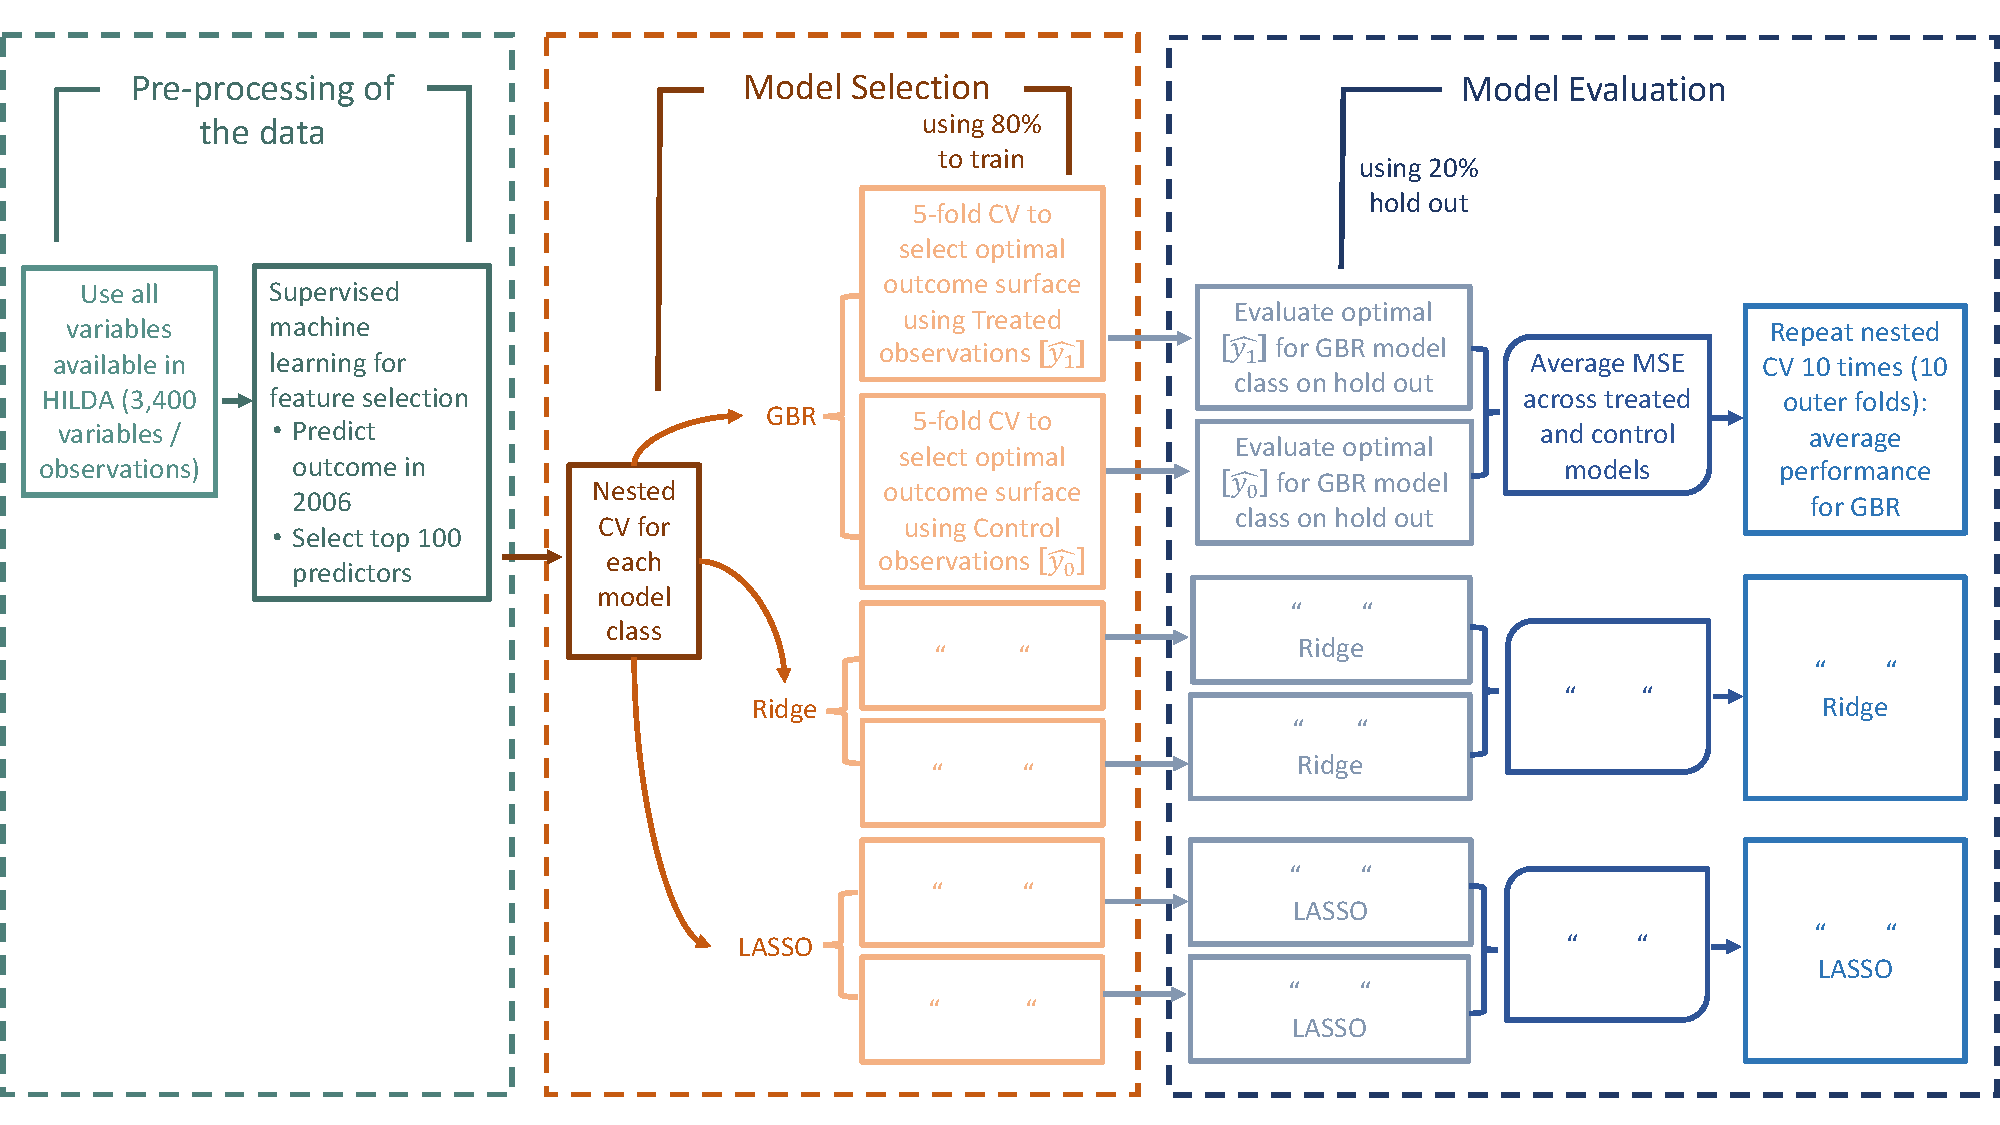
\includegraphics[scale=0.65]{_figures/explainer1.pdf}
\end{figure}

\begin{figure}[htbp]
\centering
\caption{Generating Uncertainty Parameters}
  \label{fig:exp_param}
    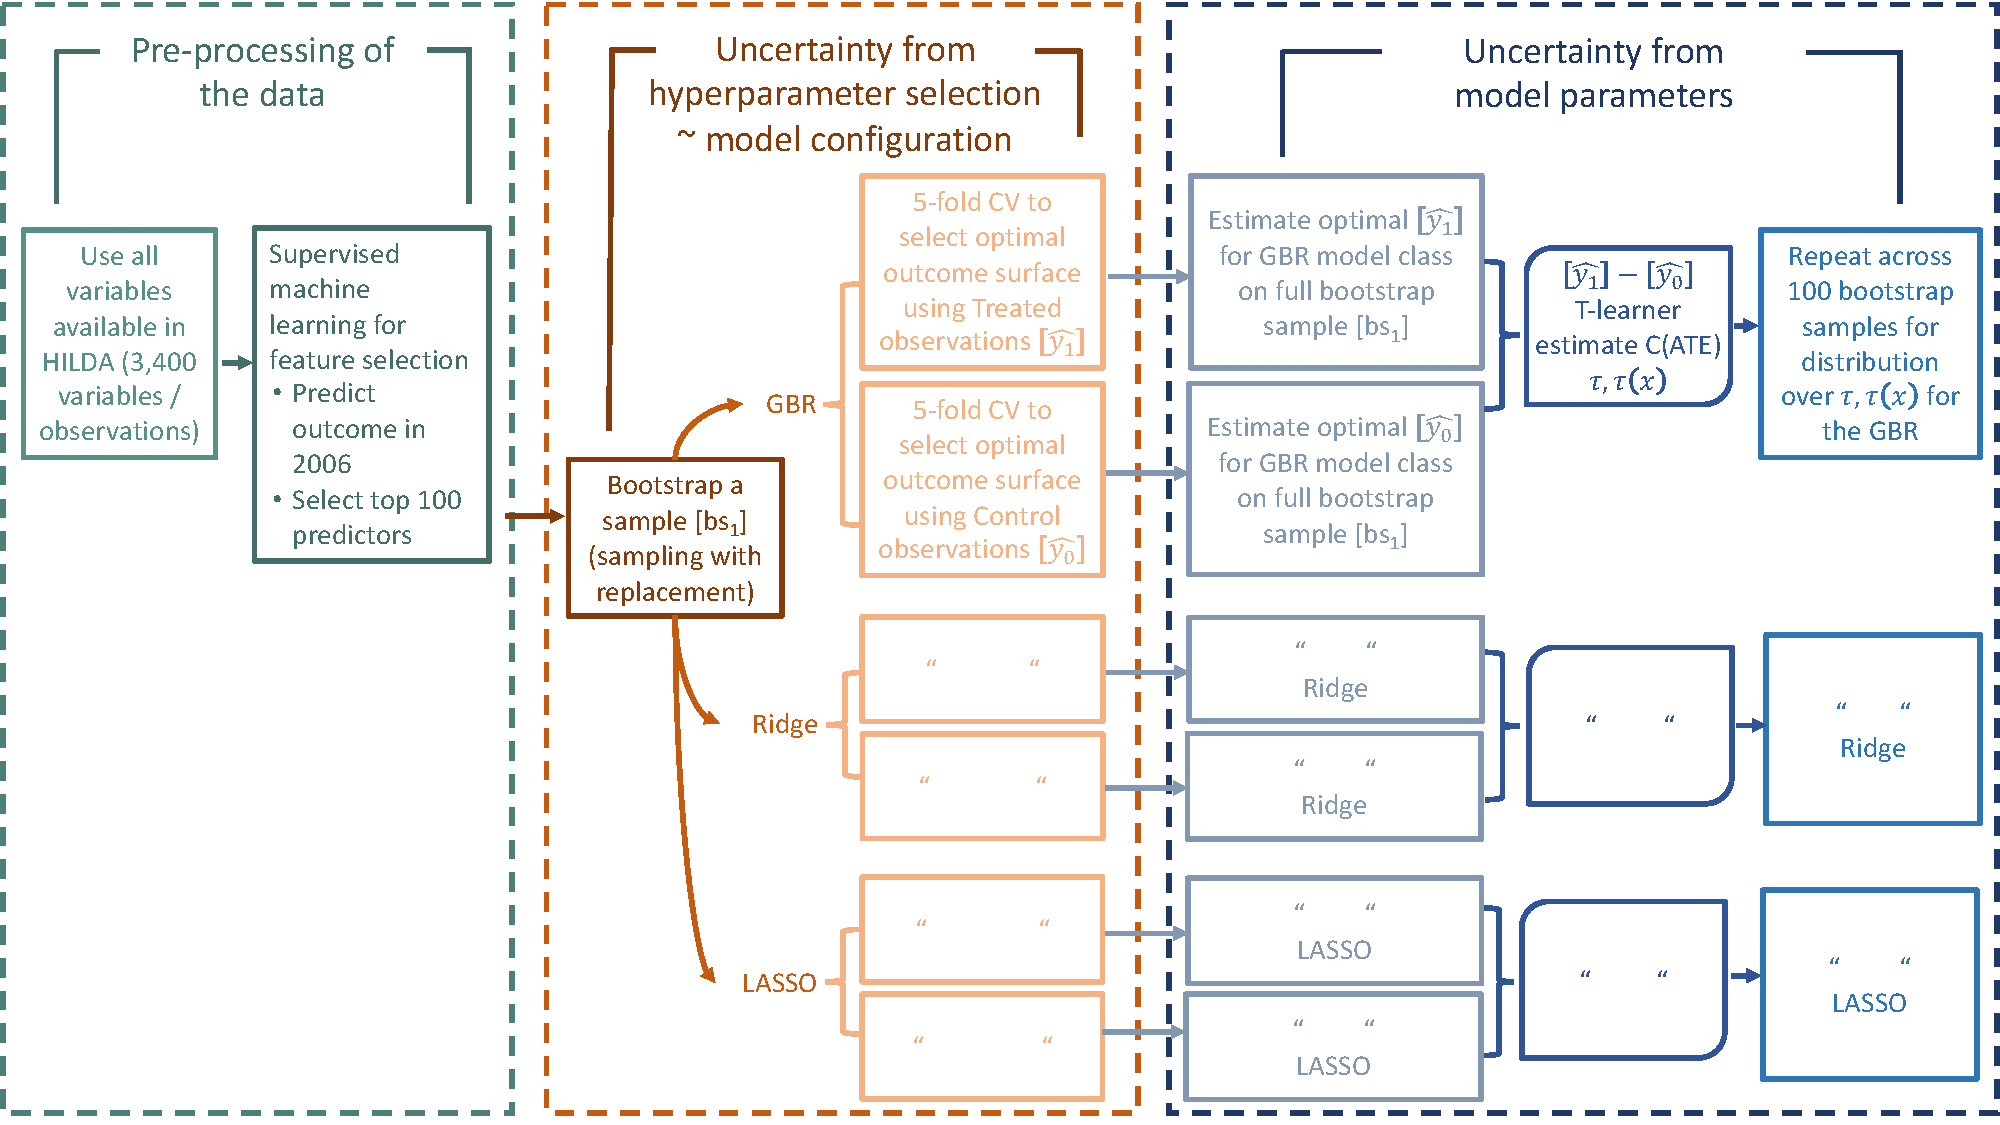
\includegraphics[scale=0.65]{_figures/explainer2.pdf}
\end{figure}


\end{landscape} 


% Descriptive figures
\begin{figure}[htbp]
\centering
\caption{Timing of Completion}
\vspace{0.5cm}
  \label{fig:yearcomp}
    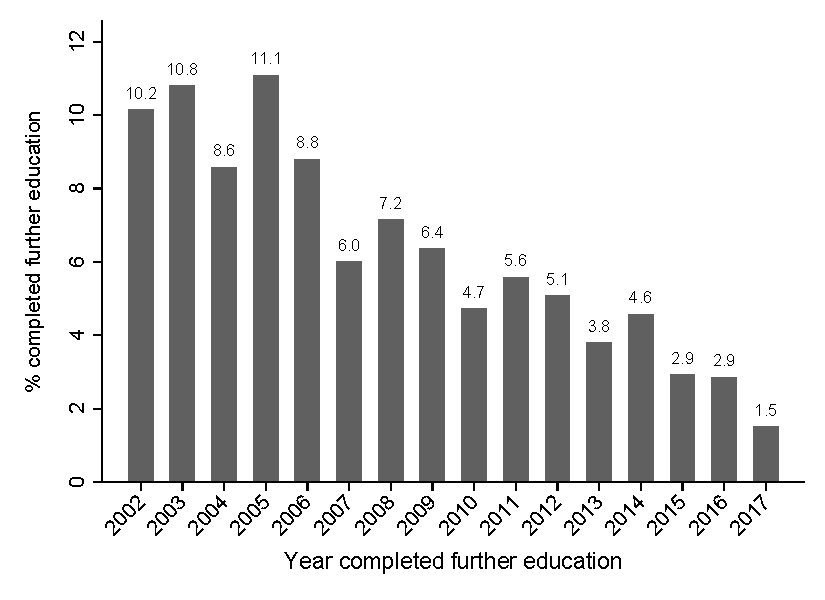
\includegraphics{_figures/year_completed.pdf}
    \parbox{1\textwidth}{\footnotesize{\textit{Notes}: Sample of 25 or older respondents who had completed a degree at any point between 2002 and 2017. Total completions: 1,383.}}
\end{figure}

\begin{figure}[htbp]
\centering
\caption{Degree completions by age}
\vspace{0.5cm}
  \label{fig:degbyage}
    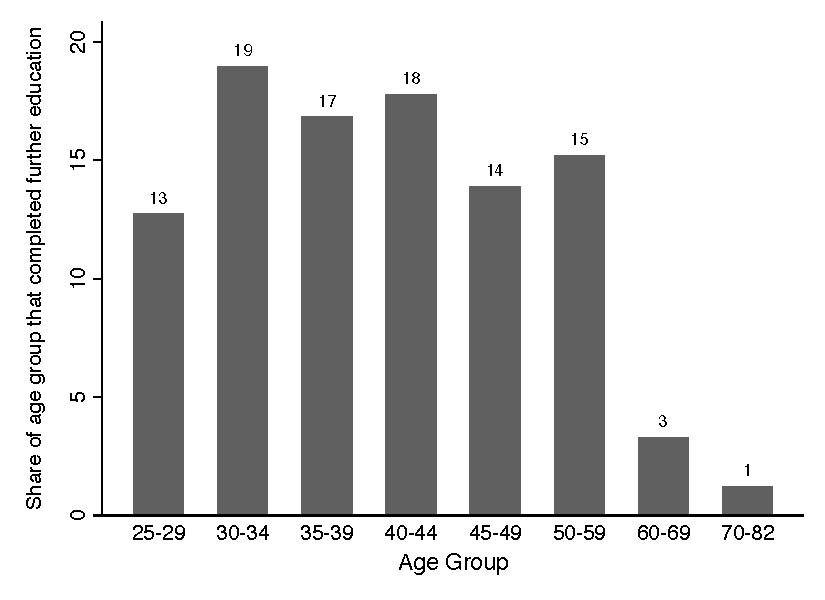
\includegraphics{_figures/descriptive_fig3b_bw.pdf}
\end{figure}

\begin{figure}[htbp]
\centering
\caption{Timing of Completion by Type of Degree}
\vspace{0.5cm}
  \label{fig:yearcompdeg}
    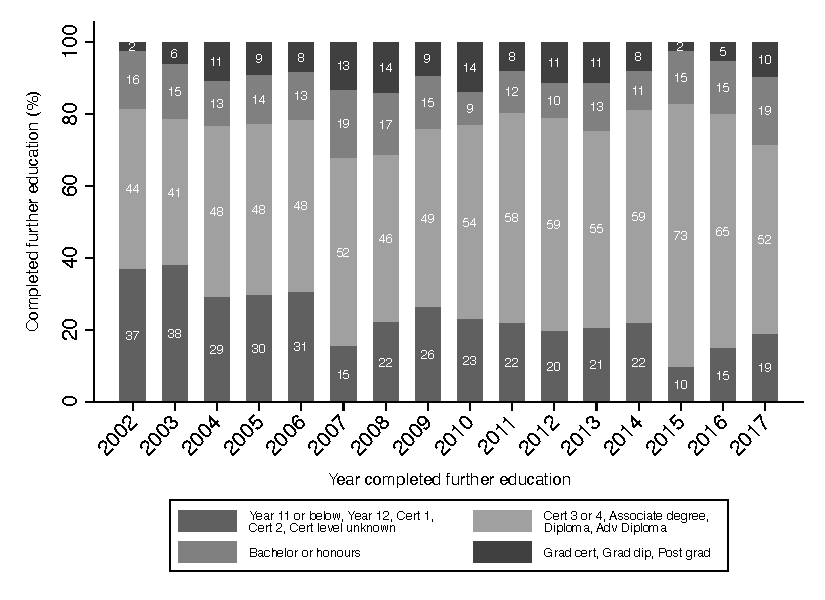
\includegraphics{_figures/year_completed_bydegree.pdf}
\parbox{1\textwidth}{\footnotesize{\textit{Notes}: Sample of 25 or older respondents who had completed a degree at any point between 2002 and 2017. Total completions: 1,383.}}
\end{figure}

%\begin{figure}[htbp]
%\centering
%\caption{Timing of Completion by Type of Degree and Gender}
%\vspace{0.5cm}
%  \label{fig:yearcompdeggen}
%    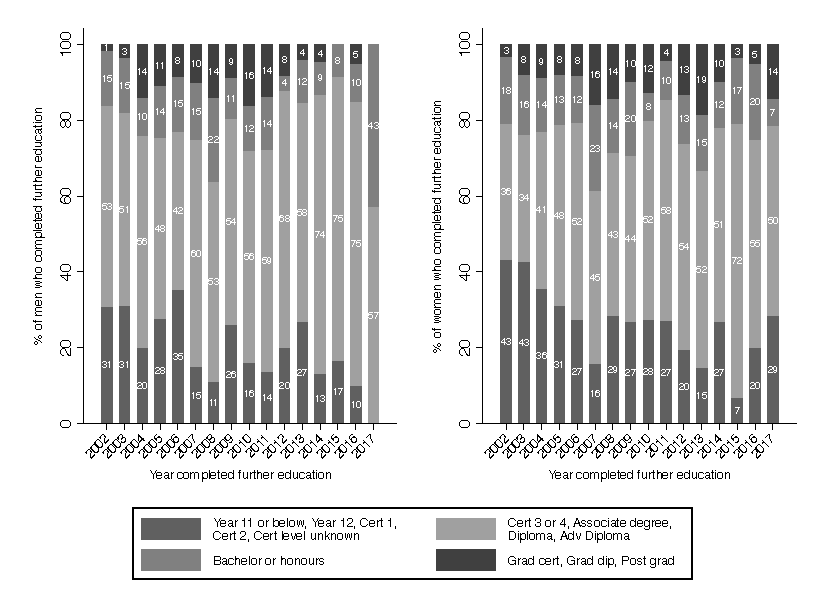
\includegraphics{_figures/year_completed_by_degree_gender.pdf}
%\parbox{1\textwidth}{\footnotesize{\textit{Notes}: Sample of 25 or older respondents who had completed a degree at any point between 2002 and 2017. Total completions: 1,383.}}
%\end{figure}

\begin{figure}[htbp]
\centering
\caption{Degree completions by sex}
\vspace{0.5cm}
  \label{fig:degbysex}
    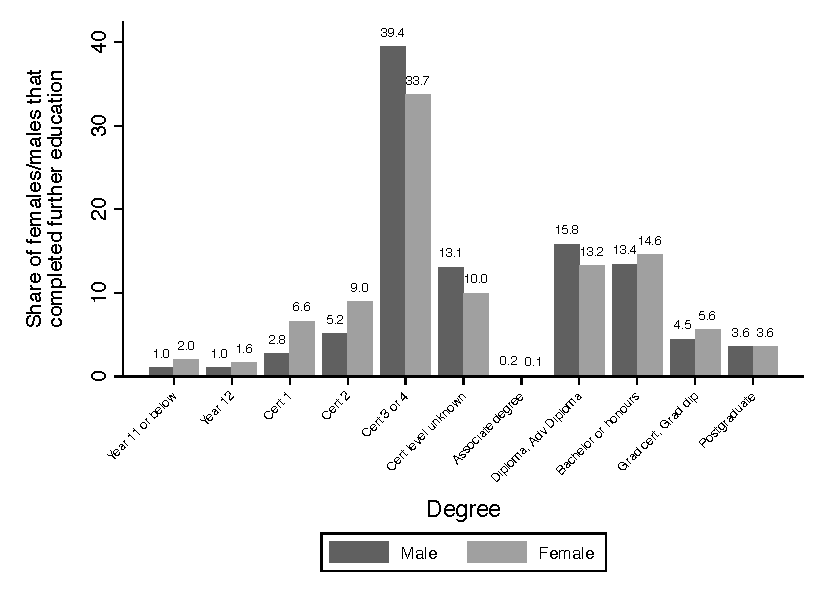
\includegraphics{_figures/completions_by_gender_deg.pdf}
\end{figure}

\begin{figure}[htbp]
\centering
\caption{Earnings and Employment by year}
\vspace{0.5cm}
  \label{fig:yearearnempl}
    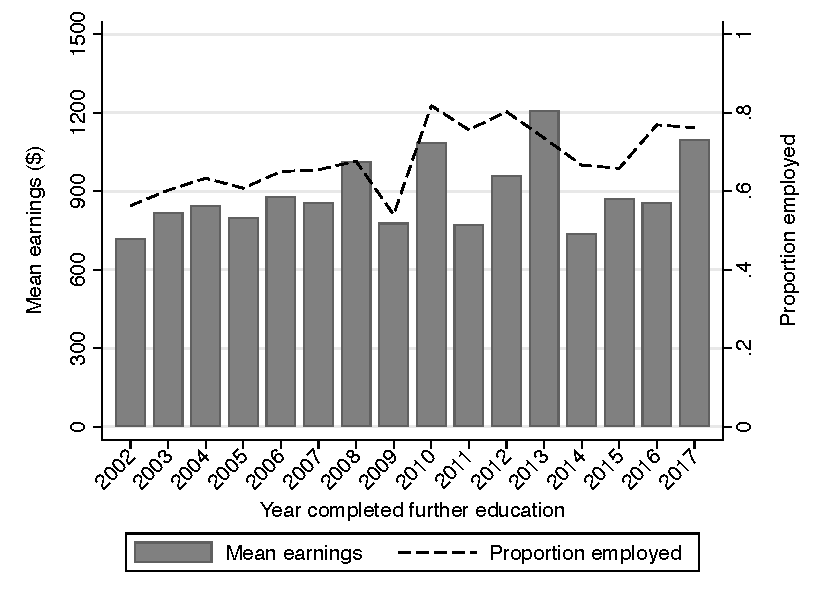
\includegraphics{_figures/mean_earnings_empl_year.pdf}
\end{figure}

%\begin{figure}[htbp]
%\centering
%\caption{Earnings and Employment by year and sex}
%\vspace{0.5cm}
%  \label{fig:sexearnempl}
%    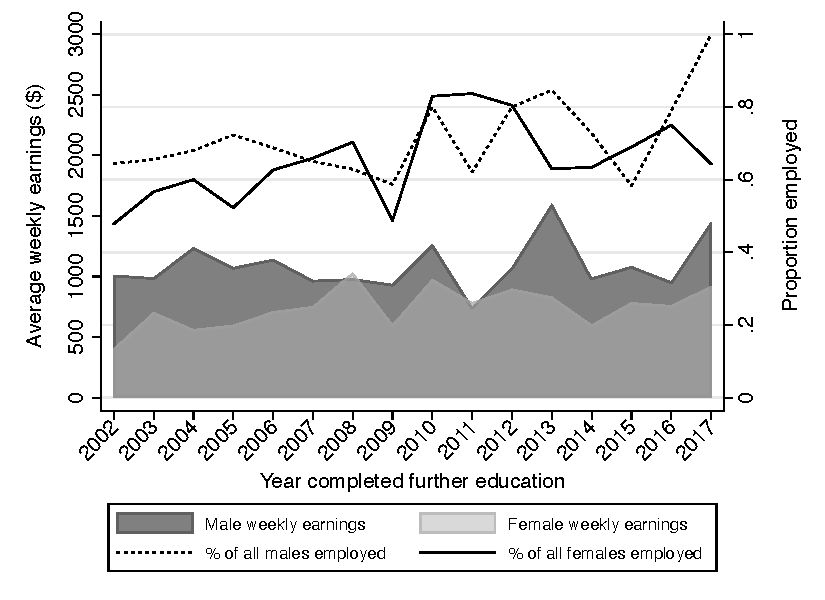
\includegraphics{_figures/mean_earnings_empl_bysex.pdf}
%\end{figure}

% \clearpage
%\begin{figure}[htbp]
%\centering
%\caption{Important Features in Heterogeneous Treatment Effects Estimation using T-Learner (GBR): Level Earnings}
%\vspace{0.5cm}
%  \label{fig:featgbr}
%    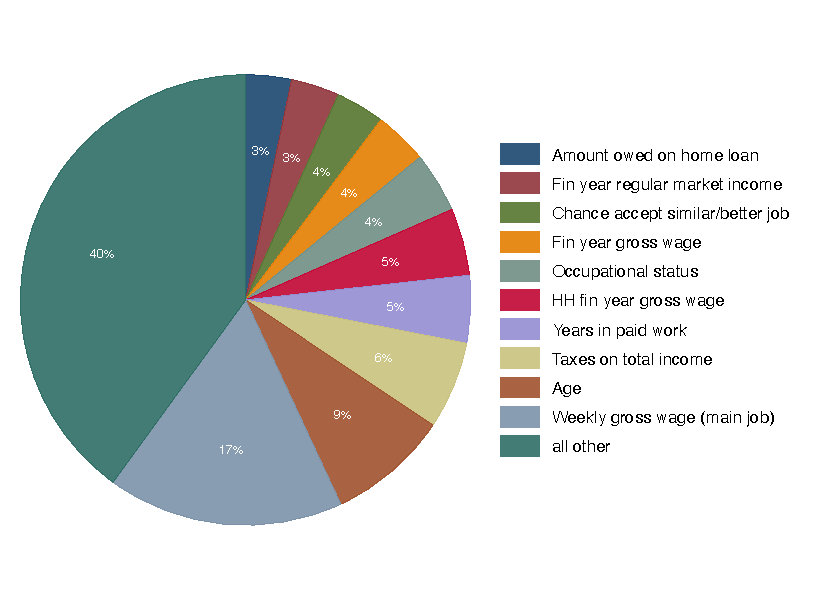
\includegraphics{_figures/influenceP_GBR_le_100.pdf}
%\parbox{1\textwidth}{\footnotesize{\textit{Notes}: Sample of 25 or older who had completed a degree at any point between 2002 and 2017. Total number of observations 5,441.}}
%\end{figure}
%
%\begin{figure}[htbp]
%\centering
%\caption{Top 3 Features Distribution of Importance using T-Learner: Level Earnings}
%\vspace{0.5cm}
%  \label{fig:dengbrlev}
%    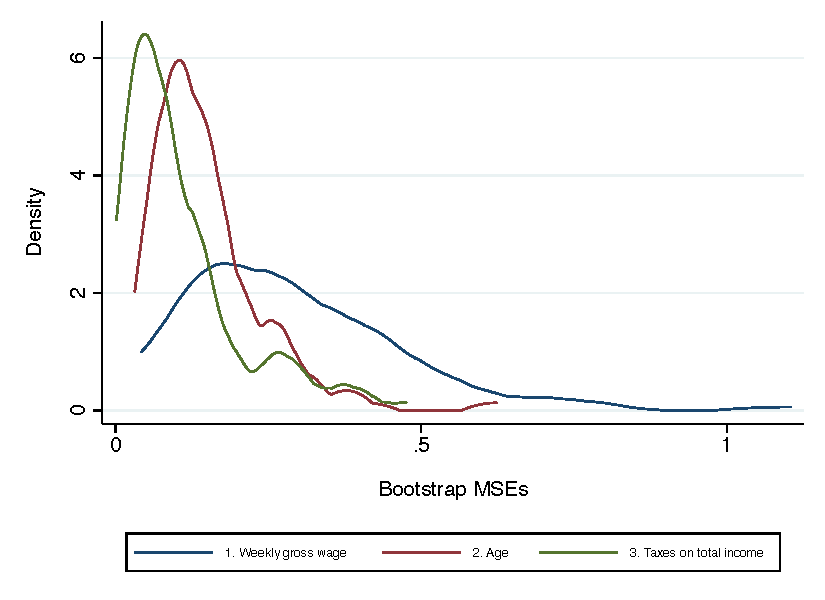
\includegraphics{_figures/density_GBR_le_100_top3.pdf}
%\parbox{1\textwidth}{\footnotesize{\textit{Notes}: Sample of 25 or older who had completed a degree at any point between 2002 and 2017. Total number of observations 5,441.}}
%\end{figure}
%
%\begin{figure}[htbp]
%\centering
%\caption{Top and Middle 3 Features Distribution of Importance using T-Learner: Level Earnings}
%\vspace{0.5cm}
%  \label{fig:dengbrlevtopmid3}
%    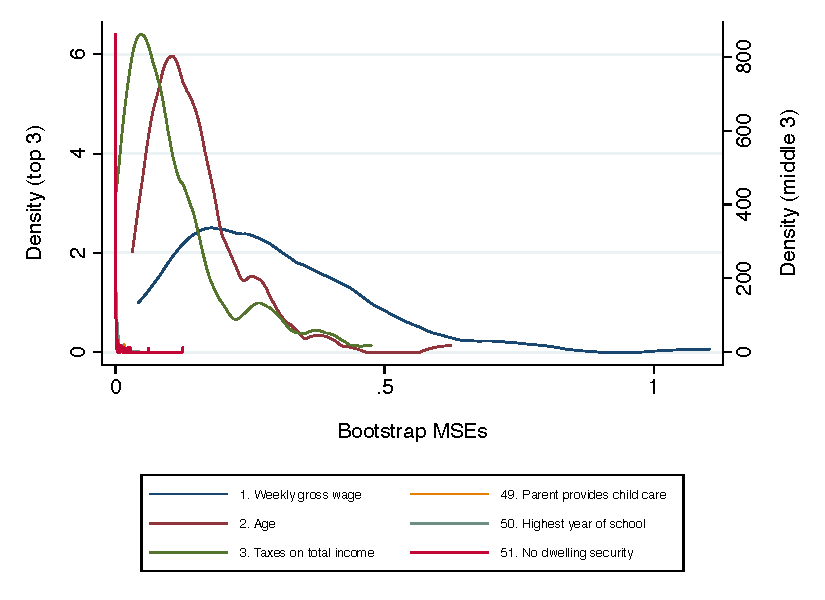
\includegraphics{_figures/density_GBR_le_100_top3mid3.pdf}
%\parbox{1\textwidth}{\footnotesize{\textit{Notes}: Sample of 25 or older who had completed a degree at any point between 2002 and 2017. Total number of observations 5,441.}}
%\end{figure}

\begin{figure}[htbp]
\centering
\caption{Important Features in Heterogeneous Treatment Effects Estimation using DR: Level Earnings}
\vspace{0.5cm}
  \label{fig:featgbrDR}
    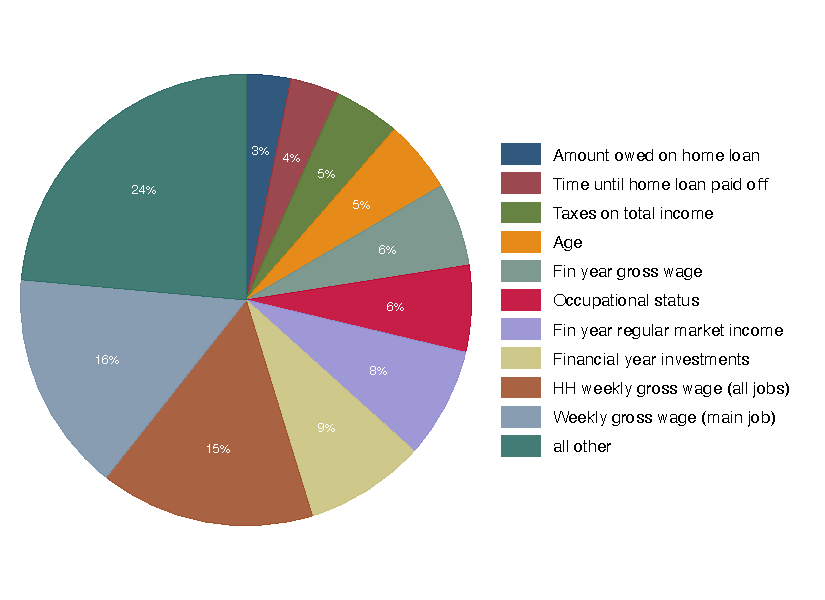
\includegraphics{_figures/DR_influenceP_GBR_le_100.pdf}
\parbox{1\textwidth}{\footnotesize{\textit{Notes}: Sample of 25 or older who had completed a degree at any point between 2002 and 2017. Total number of observations 5,441.}}
\end{figure}

\begin{figure}[htbp]
\centering
\caption{Top 3 Features Distribution of Importance using DR: Level Earnings}
\vspace{0.5cm}
  \label{fig:dengbrlevDR} 
    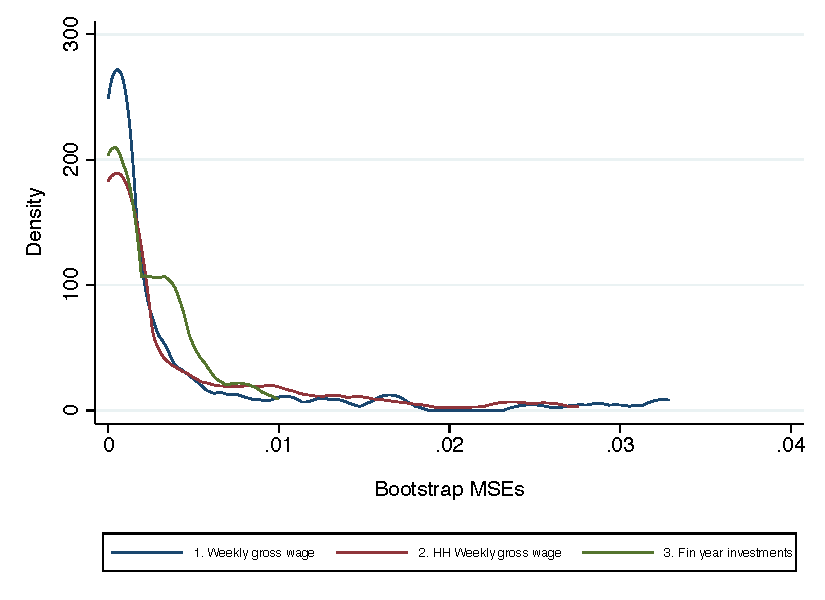
\includegraphics{_figures/density_GBR_le_100_top3_DR.pdf}
\parbox{1\textwidth}{\footnotesize{\textit{Notes}: Sample of 25 or older who had completed a degree at any point between 2002 and 2017. Total number of observations 5,441.}}
\end{figure}

%\begin{figure}[htbp]
%\centering
%\caption{Top and Middle 3 Features Distribution of Importance using DR: Level Earnings}
%\vspace{0.5cm}
%  \label{fig:dengbrlevtopmid3}
%    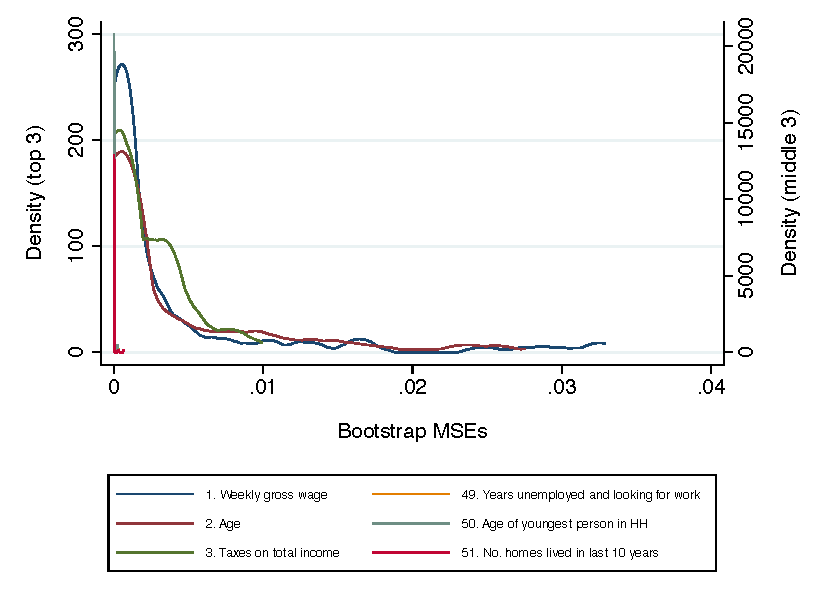
\includegraphics{_figures/density_GBR_le_100_top3mid3_DR.pdf}
%\parbox{1\textwidth}{\footnotesize{\textit{Notes}: Sample of 25 or older who had completed a degree at any point between 2002 and 2017. Total number of observations 5,441.}}
%\end{figure}



% Results
\clearpage

\begin{figure}[htbp]
\centering
\caption{Methodology}
\vspace{0.5cm}
  \label{fig:method}
    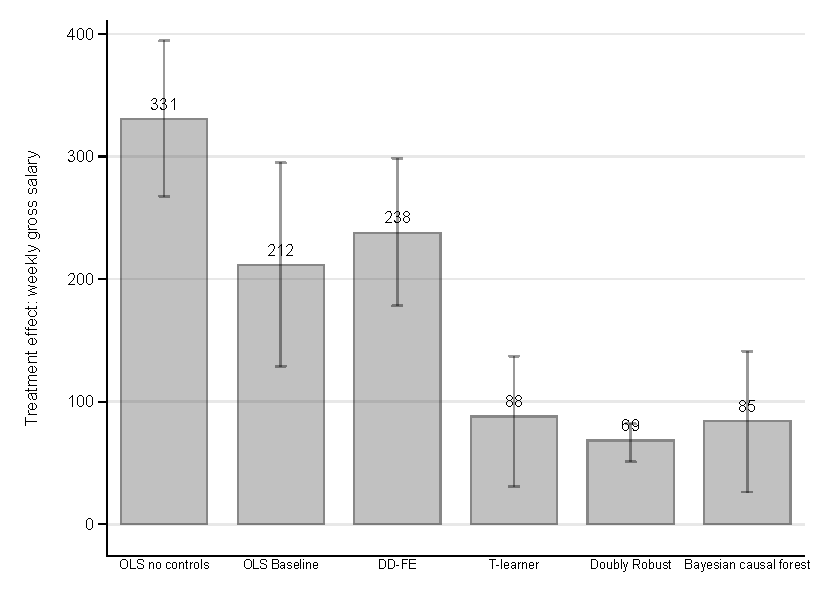
\includegraphics{_figures/method_v2.pdf}
\parbox{1\textwidth}{\footnotesize{\textit{Notes}: }}
\end{figure}

\begin{figure}[htbp]
\centering
\caption{Other Employment Outcomes}
\vspace{0.5cm}
  \label{fig:empl}
    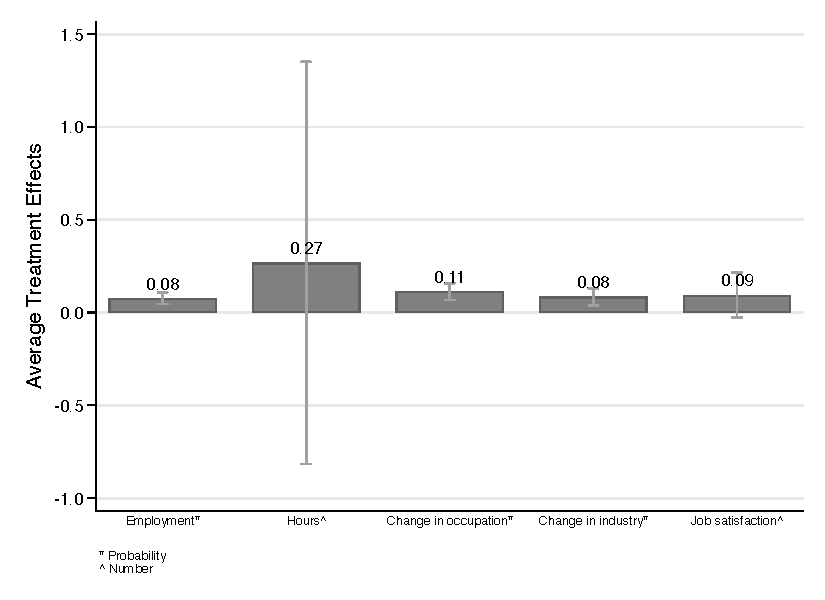
\includegraphics{_figures/SPRC_fig5_empltr.pdf}
\parbox{1\textwidth}{\footnotesize{\textit{Notes}: The impact of a new qualification. Sample of people who are 25 or older in 2001. LASSO model.}}
\end{figure}

%\begin{figure}[htbp]
%\centering
%\caption{Type of degree and subject area}
%\vspace{0.5cm}
%  \label{fig:degree}
%    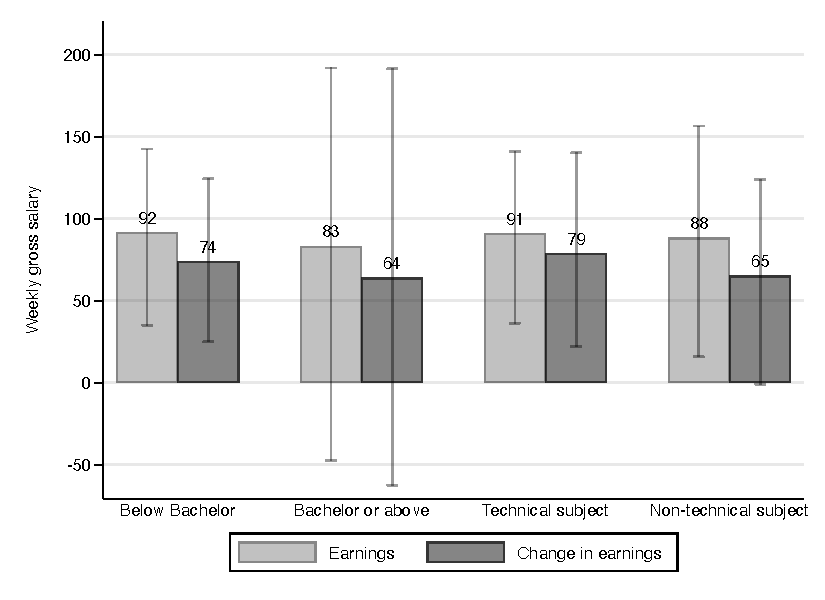
\includegraphics{_figures/hte_bach_tech.pdf}
%\parbox{1\textwidth}{\footnotesize{\textit{Notes}: }}
%\end{figure}
%
%\begin{figure}[htbp]
%\centering
%\caption{Heterogenous Treatment Effects: Demographics}
%\vspace{0.5cm}
%  \label{fig:demo}
%    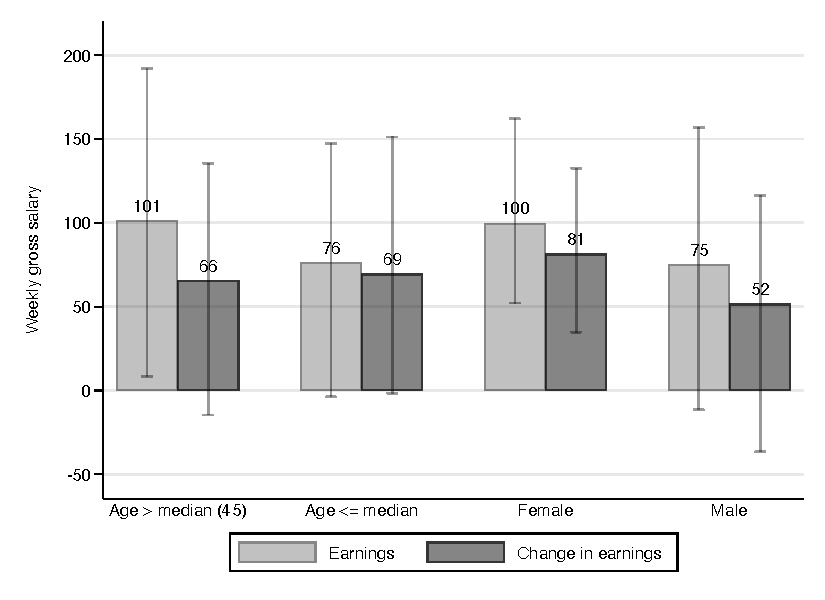
\includegraphics{_figures/hte_demographics.pdf}
%\parbox{1\textwidth}{\footnotesize{\textit{Notes}: }}
%\end{figure}
%
%\begin{figure}[htbp]
%\centering
%\caption{Heterogenous Treatment Effects: SES background}
%\vspace{0.5cm}
%  \label{fig:ses}
%    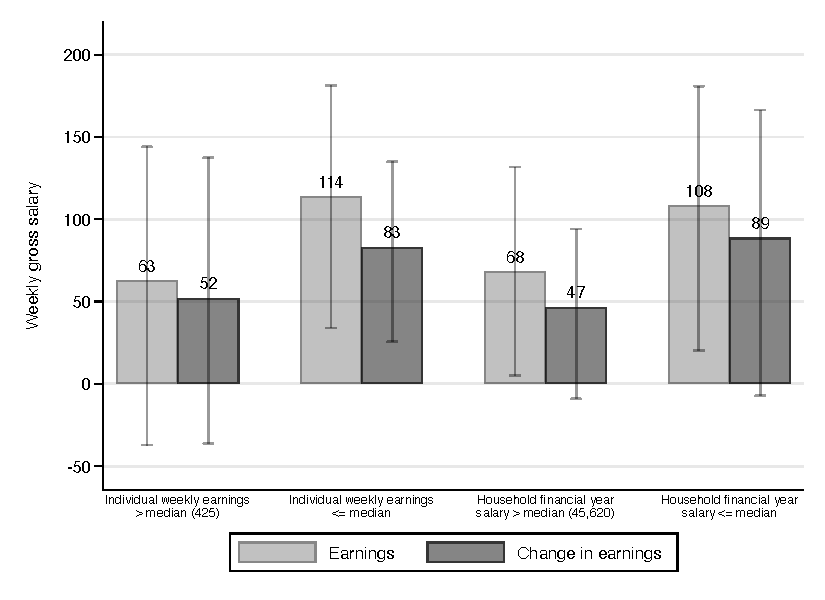
\includegraphics{_figures/hte_background.pdf}
%\parbox{1\textwidth}{\footnotesize{\textit{Notes}: }}
%\end{figure}

%\begin{figure}[htbp]
%\centering
%\caption{Earnings HTEs: GBR}
%\vspace{0.5cm}
%  \label{fig:htegbr}
%    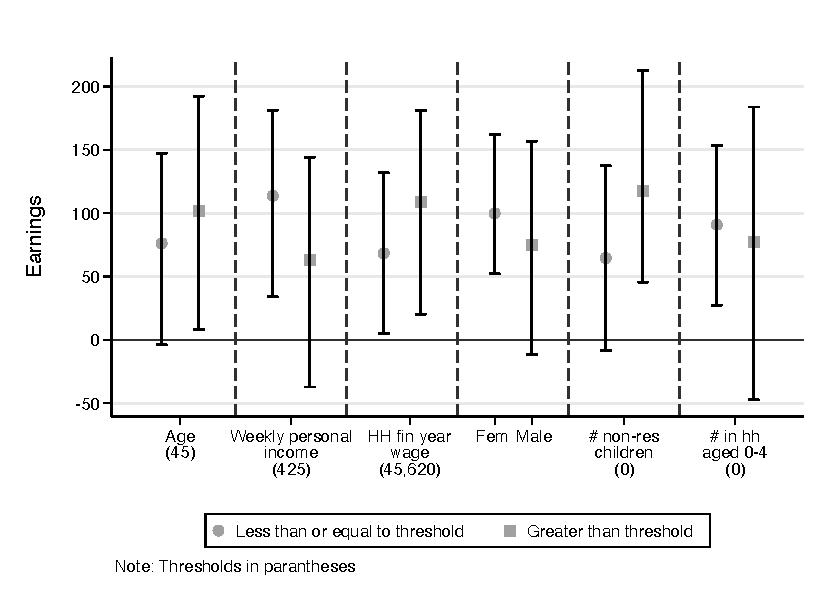
\includegraphics{_figures/hte_earnings_GL_100.pdf}
%\parbox{1\textwidth}{\footnotesize{\textit{Notes}: Sample of 25 or older who had completed a degree at any point between 2002 and 2017. Total number of observations 5,441.}}
%\end{figure}

%\begin{figure}[htbp]
%\centering
%\caption{Earnings HTEs: LASSO}
%\vspace{0.5cm}
%  \label{fig:htelasso}
%    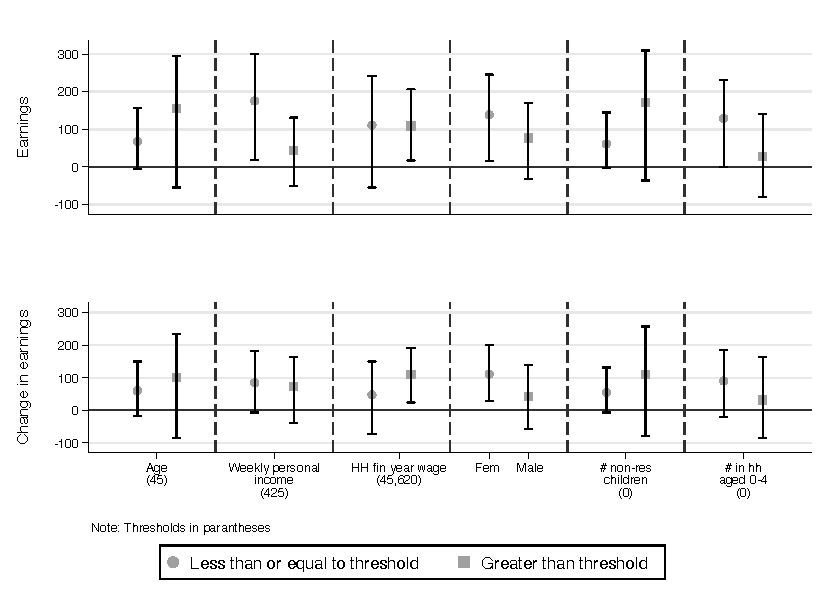
\includegraphics{_figures/hte_earnings_L_100.pdf}
%\parbox{1\textwidth}{\footnotesize{\textit{Notes}: }}
%\end{figure}
%
%\begin{figure}[htbp]
%\centering
%\caption{Earnings HTEs: Ridge}
%\vspace{0.5cm}
%  \label{fig:hteridge}
%    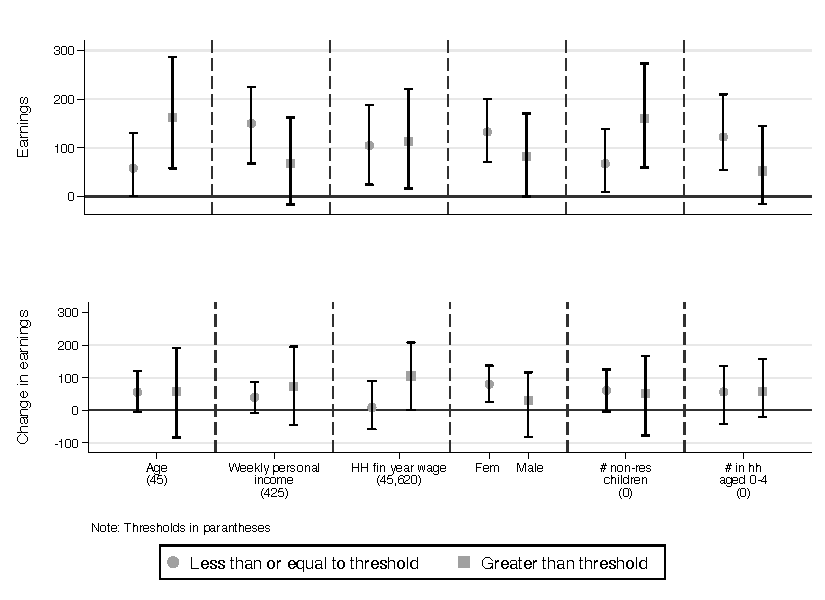
\includegraphics{_figures/hte_earnings_R_100.pdf}
%\parbox{1\textwidth}{\footnotesize{\textit{Notes}: }}
%\end{figure}

\begin{figure}[htbp]
\centering
\caption{Earnings HTEs: DR}
\vspace{0.5cm}
  \label{fig:htedr}
    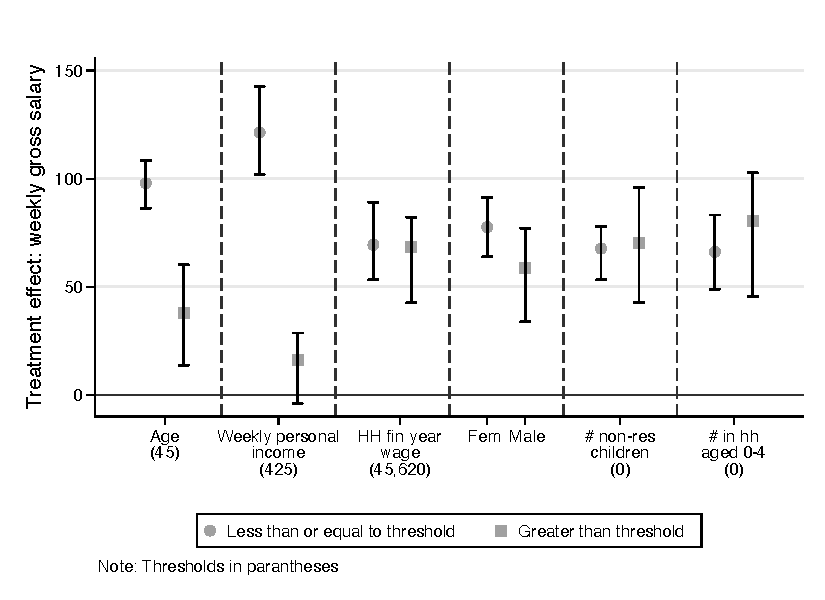
\includegraphics{_figures/hte_earnings_GL_100_DR.pdf}
\parbox{1\textwidth}{\footnotesize{\textit{Notes}: Sample of 25 or older who had completed a degree at any point between 2002 and 2017. Total number of observations 5,441.}}
\end{figure}

%\begin{figure}[htbp]
%\centering
%\caption{Earnings HTEs: ML and DR}
%\vspace{0.5cm}
%  \label{fig:htemldr}
%    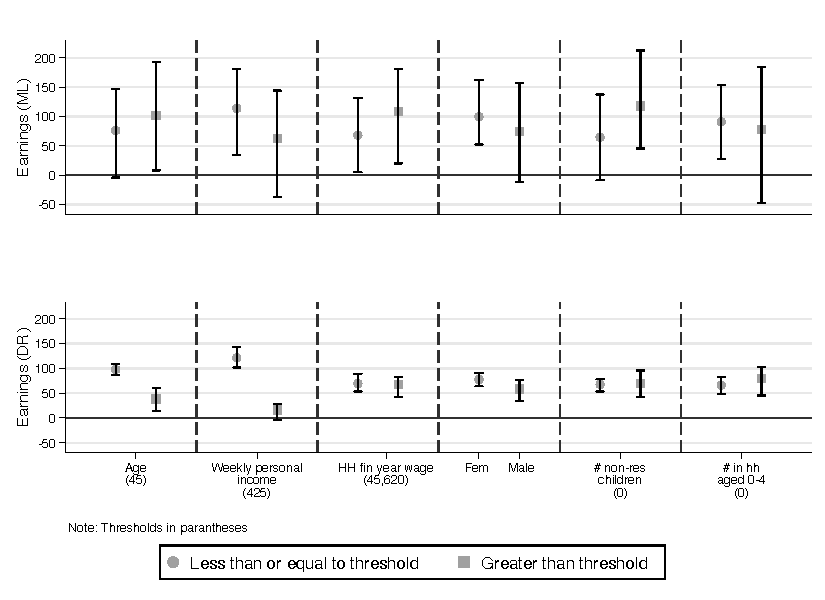
\includegraphics{_figures/hte_earnings_GL_100_MLvDR.pdf}
%\parbox{1\textwidth}{\footnotesize{\textit{Notes}: }}
%\end{figure}


\clearpage
\bibliographystyle{aea}
\bibliography{reed.bib}
%\renewcommand*{\bibfont}{\small}
%\printbibliography 
%\appendix
%\normalsize
%\setcounter{table}{0}
%\renewcommand{\thetable}{A\arabic{table}}


\clearpage
\section{Appendix}
%
%\begin{figure}[htbp]
%\centering
%\caption{Timing of Completion by Age}
%\vspace{0.5cm}
%  \label{fig:yearcompage}
%    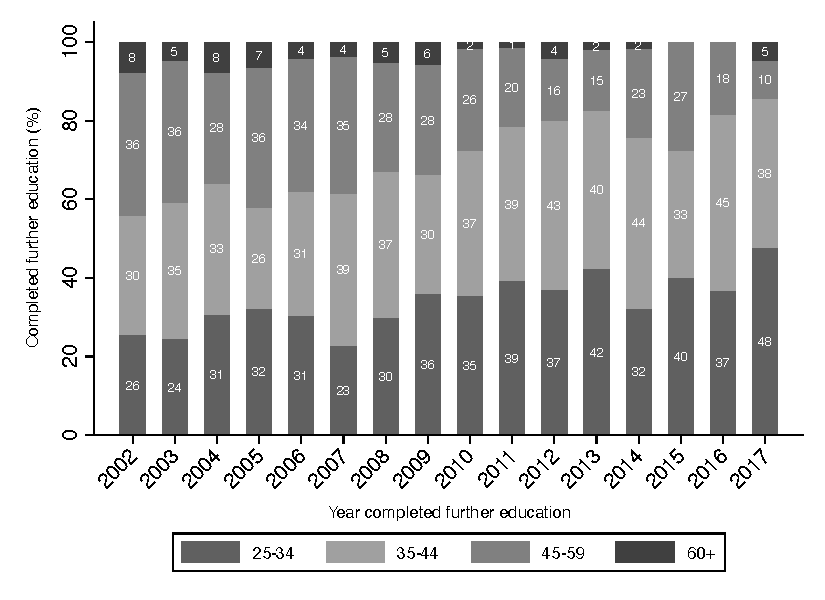
\includegraphics{_figures/year_completed_byage.pdf}
%\parbox{1\textwidth}{\footnotesize{\textit{Notes}: Sample of 25 or older respondents who had completed a degree at any point between 2002 and 2017. Total completions: 1,383.}}
%\end{figure}
%
%\begin{figure}[htbp]
%\centering
%\caption{Value-add in earnings}
%\vspace{0.5cm}
%  \label{fig:earnings}
%    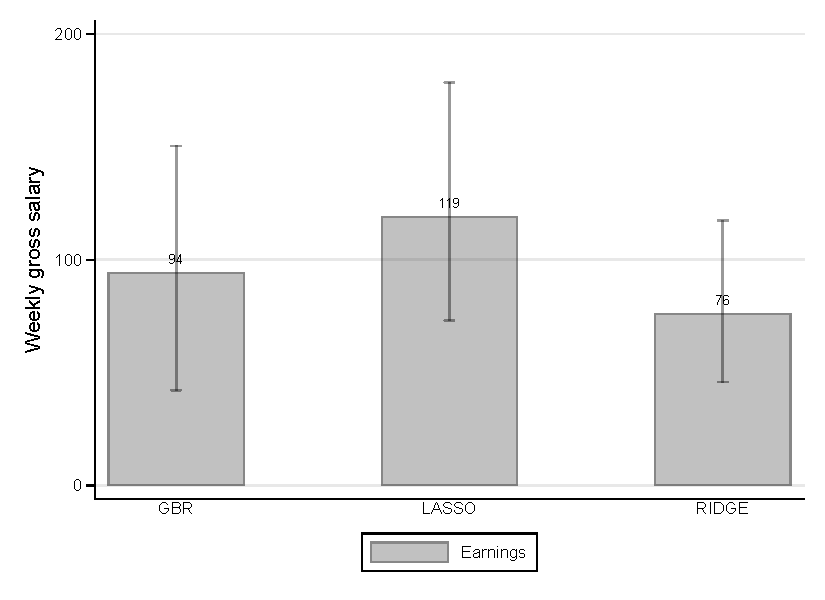
\includegraphics{_figures/valadearn.pdf}
%\parbox{1\textwidth}{\footnotesize{\textit{Notes}: }}
%\end{figure}

\begin{figure}[htbp]
\centering
\caption{Value-add in earnings: 25-45 year-old sample}
\vspace{0.5cm}
  \label{fig:valadle46}
    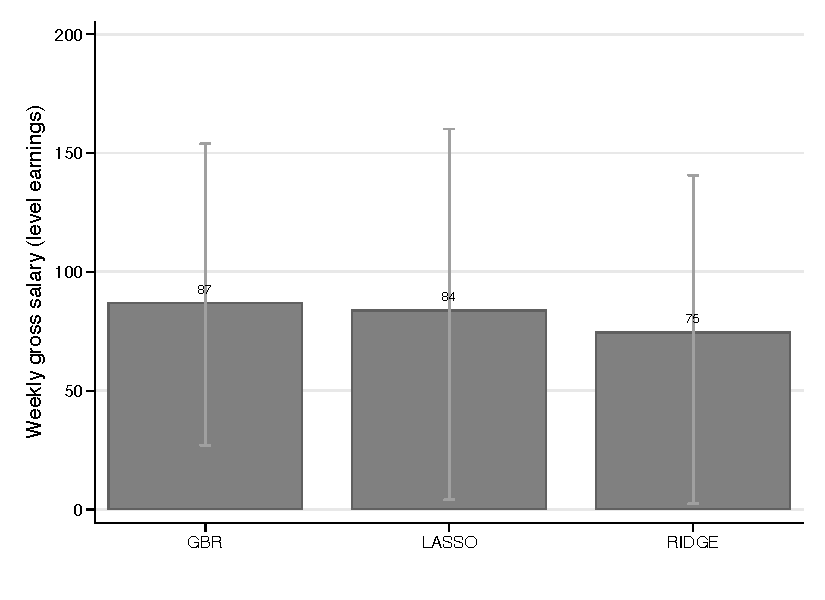
\includegraphics{_figures/valad_levearn_46.pdf}
\parbox{1\textwidth}{\footnotesize{\textit{Notes}: Sample of 25-45 who had completed a degree at any point between 2002 and 2017. Total number of observations 3,684.}}
\end{figure}

\begin{figure}[htbp]
\centering
\caption{Value-add in log earnings}
\vspace{0.5cm}
  \label{fig:valadlelog}
    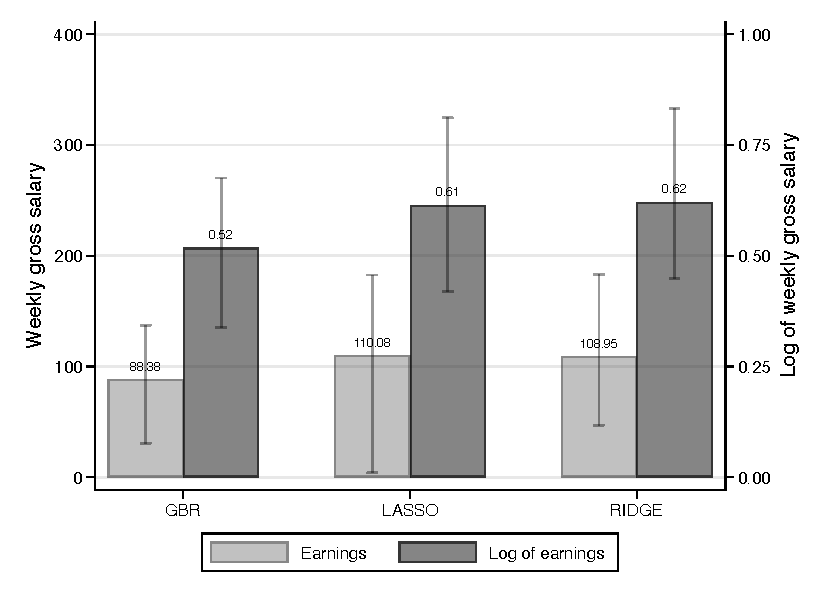
\includegraphics{_figures/valad_levearn_log.pdf}
\parbox{1\textwidth}{\footnotesize{\textit{Notes}: Sample of 25 or older who had completed a degree at any point between 2002 and 2017. Total number of observations 5,441.}}
\end{figure}
%
%% Pie charts RIDGE and LASSO
%\begin{figure}[htbp]
%\centering
%\caption{Important Features in Heterogeneous Treatment Effects Estimation using RIDGE: Level Earnings}
%\vspace{0.5cm}
%  \label{fig:featridge}
%    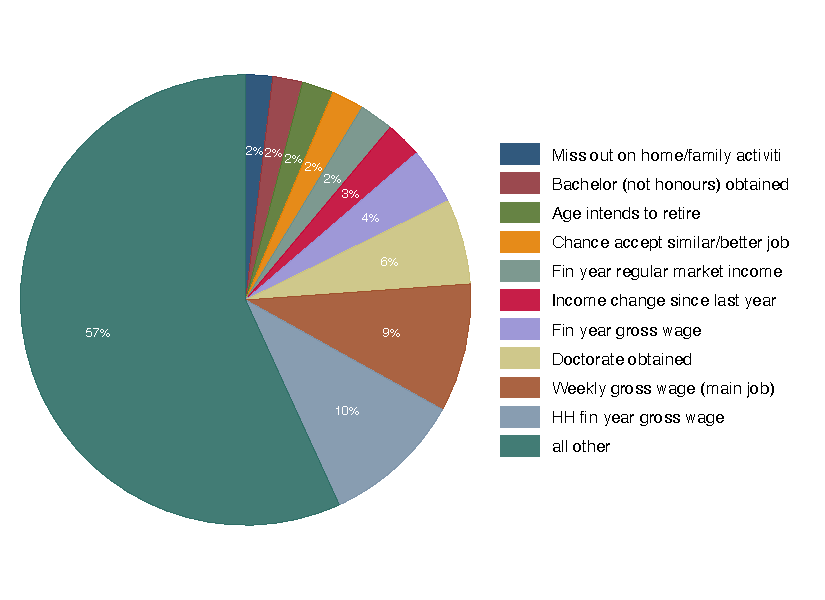
\includegraphics{_figures/influenceP_RIDGE_le_100.pdf}
%\parbox{1\textwidth}{\footnotesize{\textit{Notes}: Sample of 25 or older who had completed a degree at any point between 2002 and 2017. Total number of observations 5,441.}}
%\end{figure}
%
%\begin{figure}[htbp]
%\centering
%\caption{Important Features in Heterogeneous Treatment Effects Estimation using LASSO: Level Earnings}
%\vspace{0.5cm}
%  \label{fig:featlasso}
%    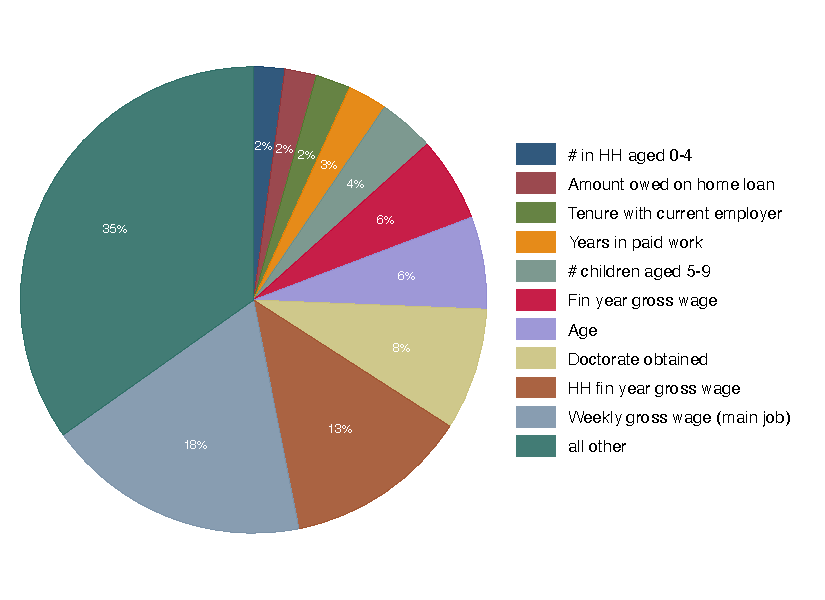
\includegraphics{_figures/influenceP_LASSO_le_100.pdf}
%\parbox{1\textwidth}{\footnotesize{\textit{Notes}: Sample of 25 or older who had completed a degree at any point between 2002 and 2017. Total number of observations 5,441.}}
%\end{figure}
%


\begin{figure}[htbp]
\centering
\caption{Important Features in Heterogeneous Treatment Effects Estimation using T-Learner (GBR): Level Earnings}
\vspace{0.5cm}
  \label{fig:featgbr}
    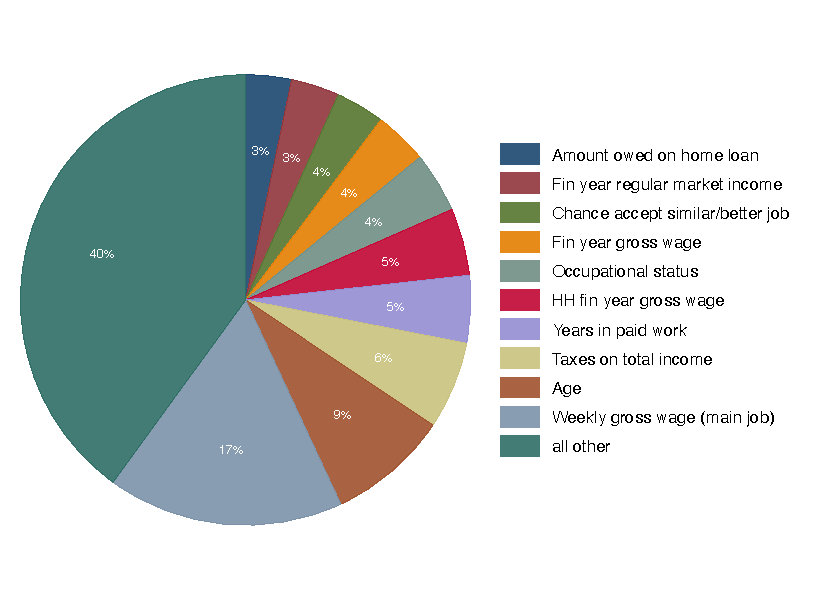
\includegraphics{_figures/influenceP_GBR_le_100.pdf}
\parbox{1\textwidth}{\footnotesize{\textit{Notes}: Sample of 25 or older who had completed a degree at any point between 2002 and 2017. Total number of observations 5,441.}}
\end{figure}


%
%\begin{landscape}  
%
%% Table 3 change in earnings section
%\clearpage
%\begin{table}[htbp]
%\centering
%\small
%\caption{Nested CV Holdout Sample: Change in Earnings}
%\begin{tabular}{cccccccc}
%\toprule
%Model   &  Outcome surface  &  Negative MSE  &  NMSE Std  &  R-squared  &  R-squared Std  & ATE   & ATE\_std   \\
%\midrule                               																		
%\multirow{2}{*}{\hfil GBR}	& 	Treated	 &  -1013520  &  389355  &  0.13  &  0.11  & 	\multirow{2}{*}{\hfil 	53.2	} & \multirow{2}{*}{\hfil 20.4	}	 \\
%& 	Control	 & -664787	 & 113211	& 	0.25  &  0.06  & & \\
%\midrule       																				
%\multirow{2}{*}{\hfil LASSO}	 &  Treated &  -981927  & 	364876  & 0.15  &  0.10  &  \multirow{2}{*}{\hfil  73.1 }  &  \multirow{2}{*}{\hfil 19.7}  \\
%&  Control  &  -703529  & 	178858	 & 0.20  &  0.07  & & \\
%\midrule      	     	    									
%\multirow{2}{*}{\hfil Ridge}	 & Treated	 & -1004753	 & 446164  &  0.15  & 0.09 &  \multirow{2}{*}{\hfil 43.7} & \multirow{2}{*}{\hfil 11.0}	 \\
%& 	Control	& -708521 & 174065	& 0.20	& 0.05	 & & \\
%\midrule
%\bottomrule
%\end{tabular}
%\par\medskip
%\parbox{1.3\textwidth}{\footnotesize Notes: 5 fold CV performed on 80\% train sample. All statistics presented in this table are based on the 20\% holdout sample. Ten outer folds are used. See Figure \ref{fig:exp_model} for more details}. \\
%\label{tab:ncvhosce}
%\end{table}
%
%
%
%% Table 5 change in earnings section
%% Bootstrapped ATEs
%\newcolumntype{C}[1]{>{\centering\arraybackslash}m{#1}} % center columns horizontally and vertically 
%\clearpage
%\begin{table}[htbp]
%\centering
%\small
%\caption{Average Treatment Effects: Change in Earnings. Comparisons across models.}
%\begin{tabular}{p{0.5\textwidth} C{0.1\textwidth} C{0.1\textwidth} C{0.1\textwidth}}
%\toprule
%Model	 & 	N	 & 	ATE	 & 	S.E (ATE)	 \\
%\midrule											
%OLS	 & 	5441	 & 	57.33	 & 	28.61	 \\
%T-learner (GBR)	 & 	5441	 & 	67.62	 & 	32.85	 \\
%T-learner (LASSO)	 & 	5441	 & 	79.10	 & 	46.08	 \\
%T-learner (Ridge)	 & 	5441	 & 	56.67	 & 	42.86	 \\
%Doubly Robust (GBR)	 & 	5441	 & 	60.44	 & 	10.89	 \\
%Doubly Robust (LASSO)	 & 	5441	 & 	65.20	 & 	5.33	 \\
%Doubly Robust (Ridge)	 & 	5441	 & 	63.69	 & 	3.48	 \\
%Bayesian Ridge 	 & 	5441	 & 	44.17	 & 	24.11	 \\
%Bayesian Ridge (cf. s)	 & 	5441	 & 	41.08	 & 	22.70	 \\
%Gaussian Process	 & 	5441	 & 	0.52	 & 	7.06	 \\
%Hierarchical BLM	 & 	5441	 & 	0.20	 &  \\
%\bottomrule
%\end{tabular}
%\par\medskip
%\parbox{1.1\textwidth}{\footnotesize Notes: Sample of 25 or older respondents who had completed a degree at any point between 2002 and 2017. Total completions: 1,383. See Figure \ref{fig:exp_param} for more details.}
%\label{tab:atebsch}
%\end{table}
%
%\end{landscape}  

% Density graphs RIDGE and LASSO  (UNCOMMENT WHEN GRAPHS HAVE BEEN MADE)
%\begin{figure}[htbp]
%\centering
%\caption{Top 3 features bootstrapped mean MSEs using RIDGE: Level Earnings}
%\vspace{0.5cm}
%  \label{fig:denridgelev}
%    \includegraphics{_figures/density_RIDGE_le_100.pdf}
%\parbox{1\textwidth}{\footnotesize{\textit{Notes}: \color{red} check figure title}}
%\end{figure}
%
%\begin{figure}[htbp]
%\centering
%\caption{Top 3 features bootstrapped mean MSEs using RIDGE: Change in Earnings}
%\vspace{0.5cm}
%  \label{fig:denridgech}
%    \includegraphics{_figures/density_RIDGE_ce_100.pdf}
%\parbox{1\textwidth}{\footnotesize{\textit{Notes}: \color{red} check figure title}}
%\end{figure}
%
%\begin{figure}[htbp]
%\centering
%\caption{Top 3 features bootstrapped mean MSEs using LASSO: Level Earnings}
%\vspace{0.5cm}
%  \label{fig:denlassolev}
%    \includegraphics{_figures/density_LASSO_le_100.pdf}
%\parbox{1\textwidth}{\footnotesize{\textit{Notes}: \color{red} check figure title}}
%\end{figure}
%
%\begin{figure}[htbp]
%\centering
%\caption{Top 3 features bootstrapped mean MSEs using LASSO: Change in Earnings}
%\vspace{0.5cm}
%  \label{fig:denlassoch}
%    \includegraphics{_figures/density_LASSO_ce_100.pdf}
%\parbox{1\textwidth}{\footnotesize{\textit{Notes}: \color{red} check figure title}}
%\end{figure}


\end{document}


% Table 2 (OLD VERSION)
%\clearpage    
%\begin{longtable}{p{0.5\textwidth} C{0.2\textwidth} C{0.2\textwidth} C{0.2\textwidth} C{0.2\textwidth}}
%\caption{ML variables omitted by OLS theory model} \\ 
%\hline 
%Variable label & Variable name & Relationship with re-education (redufl) & Relationship with outcome (y\_wscei) & Bias direction in OLS models \\
%\hline
%\endfirsthead
%\multicolumn{5}{c}{\textit{Continued from previous page}} \\
%\hline
%Variable label & Variable name & Relationship with re-education (redufl) & Relationship with outcome (y\_wscei) & Bias direction in OLS models \\
%\hline
%\endhead
%\hline \multicolumn{5}{r}{\textit{Continued on next page}} \\
%\endfoot
%\hline
%\endlastfoot    
%\textbf{Outcomes} & & & & \\
%Annual Earnings individual in 2019 \color{red} check this 	& 	y\_wscei	 & 	+	 & 	+	 & 	+	\\
%Employment status individual in 2019 	& 	employ01	 & 	+	 & 	+	 & 	+	\\
%Mental health 2019 	& 	y\_ghmh	 & 	-	 & 	+	 & 	-	\\
%Change in annual earnings between 2001 and 2019 \color{red} check this 	& 	y\_dwscei	 & 	+	 & 	+	 & 	+	\\
%Extra degree attained in 2002 to 2017 	& 	redufl	 & 	+	 & 	+	 & 	+	\\
%Highest level of educ changed between 2001 and 2017 	& 	reduhl	 & 	+	 & 	+	 & 	+	\\
%\textbf{Treatment Indicators} 	& 		 & 		 & 		 & 		\\
%Extra degree Bachelor and/or above 	& 	bachab	 & 	+	 & 	+	 & 	+	\\
%Below bachelor 	& 	bbach	 & 	+	 & 	+	 & 	+	\\
%Technical degree 	& 	techdeg	 & 	+	 & 	+	 & 	+	\\
%Qualitative degree* 	& 	qualdeg	 & 	+	 & 	+	 & 	+	\\
%\textbf{Covariates} 	& 		 & 		 & 		 & 		\\
%\textbf{\textit{Demographics}} 	& 		 & 		 & 		 & 		\\
%Sex 	& 	hgsex	 & 	+	 & 	-	 & 	-	\\
%Section of State 	& 	hhsos	 & 	-	 & 	-	 & 	+	\\
%Age 	& 	hgage1	 & 	-	 & 	-	 & 	+	\\
%Age of youngest person in HH 	& 	hhyng	 & 	-	 & 	-	 & 	+	\\
%No.  persons aged 0-4 years in HH 	& 	hh0\_4	 & 	+	 & 	+	 & 	+	\\
%No.  persons aged 10-14 years in HH 	& 	hh10\_14	 & 	+	 & 	+	 & 	+	\\
%Age when first left home 	& 	fmagelh	 & 	+	 & 	+	 & 	+	\\
%Living circumstances 	& 	hgms	 & 	+	 & 	-	 & 	-	\\
%English fluency 	& 	hgeab	 & 	-	 & 	-	 & 	+	\\
%Unemployment rate in region	& 	hhura	 & 	-	 & 	-	 & 	+	\\
%\textbf{\textit{Education}} 	& 		 & 		 & 		 & 		\\
%Highest year of school completed/currently attending	& 	edhists	 & 	-	 & 	-	 & 	+	\\
%Bachelor degree (without honours) obtained 	& 	edqobd	 & 	+	 & 	+	 & 	+	\\
%Masters degree obtained 	& 	edqoms	 & 	-	 & 	+	 & 	-	\\
%Doctorate obtained 	& 	edqodc	 & 	-	 & 	+	 & 	-	\\
%No.  qualifications unknown 	& 	edqunk	 & 	+	 & 	-	 & 	-	\\
%\textbf{\textit{Employment}} 	& 		 & 		 & 		 & 		\\
%Occupation 	& 	jbmo61	 & 	+	 & 	-	 & 	-	\\
%Years in paid work 	& 	ehtjbyr	 & 	-	 & 	-	 & 	+	\\
%Tenure with current employer 	& 	jbempt	 & 	-	 & 	-	 & 	+	\\
%Type of work schedule 	& 	jbmday	 & 	+	 & 	-	 & 	-	\\
%Current work schedule 	& 	jbmsch	 & 	-	 & 	-	 & 	+	\\
%Casual worker 	& 	jbcasab	 & 	-	 & 	+	 & 	-	\\
%Hours/week worked at home 	& 	jbmhrh	 & 	-	 & 	-	 & 	+	\\
%Hours/week travelling to and from work 	& 	lshrcom	 & 	+	 & 	+	 & 	+	\\
%Satisfaction with employment opportunities 	& 	losateo	 & 	-	 & 	+	 & 	-	\\
%Occupational status - current main job	& 	jbmo6s	 & 	+	 & 	+	 & 	+	\\
%No.  persons employed at place of work	& 	jbmwpsz	 & 	+	 & 	+	 & 	+	\\
%Age intends to retire 	& 	rtiage1	 & 	-	 & 	-	 & 	+	\\
%Age retired/intends to retire 	& 	rtage	 & 	+	 & 	+	 & 	+	\\
%Prob.  of losing job in next 12 months 	& 	jbmploj	 & 	-	 & 	-	 & 	+	\\
%Prob.  of accepting similar/better job 	& 	jbmpgj	 & 	+	 & 	+	 & 	+	\\
%Looked for work in last 4 weeks 	& 	jsl4wk	 & 	+	 & 	+	 & 	+	\\
%Years unemployed and looking for work	& 	ehtujyr	 & 	+	 & 	-	 & 	-	\\
%Hours per week worked in last job 	& 	ujljhru	 & 	-	 & 	-	 & 	+	\\
%Industry of last job 	& 	ujljin1	 & 	+	 & 	+	 & 	+	\\
%\textbf{\textit{Work preferences}} 	& 		 & 		 & 		 & 		\\
%Total hours per week would choose to work 	& 	jbprhr	 & 	+	 & 	+	 & 	+	\\
%Importance of work situation to your life 	& 	loimpew	 & 	+	 & 	+	 & 	+	\\
%\textbf{\textit{Childcare}} 	& 		 & 		 & 		 & 	-	\\
%Child looks after self 	& 	chu\_sf	 & 	-	 & 	-	 & 	+	\\
%Uses child care while at work	& 	cpno	 & 	-	 & 	+	 & 	-	\\
%Parent provides child care 	& 	cpu\_me 	 & 	-	 & 	-	 & 	+	\\
%\textbf{\textit{Work-family balance}} 	& 		 & 		 & 		 & 		\\
%Do fair share of looking after children 	& 	pashare	 & 	-	 & 	+	 & 	-	\\
%Miss out on home/family activities 	& 	pawkmfh	 & 	+	 & 	+	 & 	+	\\
%Working makes me a better parent 	& 	pawkbp	 & 	+	 & 	-	 & 	-	\\
%\textbf{\textit{Family}} 	& 		 & 		 & 		 & 		\\
%No.  dependent children aged 5-9 	& 	hhd5\_9	 & 	+	 & 	+	 & 	+	\\
%No.  dependent children aged 10-14 	& 	hhd1014	 & 	+	 & 	+	 & 	+	\\
%No.  non-resident children 	& 	tcnr	 & 	-	 & 	-	 & 	+	\\
%Sex of non-resident child 	& 	ncsex1	 & 	+	 & 	+	 & 	+	\\
%Likely to have a child in the future 	& 	icprob	 & 	+	 & 	+	 & 	+	\\
%\textbf{\textit{Finances}} 	& 		 & 		 & 		 & 		\\
%Owned a home previously 	& 	hspown	 & 	+	 & 	+	 & 	+	\\
%Amount outstanding on home loans 	& 	hsmgowe	 & 	+	 & 	+	 & 	+	\\
%Time until home loan paid off	& 	hsmgfin	 & 	+	 & 	+	 & 	+	\\
%Food expenses outside the home 	& 	xposml	 & 	+	 & 	+	 & 	+	\\
%SEIFA (level of economic resources) 	& 	hhec10	 & 	-	 & 	+	 & 	-	\\
%Taxes on total income 	& 	txtottp	 & 	+	 & 	+	 & 	+	\\
%Change in total gross income since 1 year ago 	& 	wslya	 & 	+	 & 	+	 & 	+	\\
%Had an incorporated business 	& 	bifinc	 & 	+	 & 	-	 & 	-	\\
%Had a non-LLC or unincorporated business 	& 	bifuinc	 & 	-	 & 	+	 & 	-	\\
%\textbf{\textit{Income}} 	& 		 & 		 & 		 & 		\\
%HH current weekly gross wages - all jobs 	& 	hiwscei	 & 	+	 & 	+	 & 	+	\\
%Current weekly gross wages - main job 	& 	wscme	 & 	+	 & 	+	 & 	+	\\
%HH financial year gross wages 	& 	hiwsfei	 & 	+	 & 	+	 & 	+	\\
%Financial year gross wages 	& 	wsfe	 & 	+	 & 	+	 & 	+	\\
%Financial year regular market income	& 	tifmktp	 & 	+	 & 	+	 & 	+	\\
%Financial year disposable total income 	& 	tifditp	 & 	+	 & 	+	 & 	+	\\
%Imputation flag: current weekly gross wages - all jobs 	& 	wscef	 & 	+	 & 	+	 & 	+	\\
%Imputation flag: current weekly gross wages - other jobs 	& 	wscoef	 & 	+	 & 	+	 & 	+	\\
%Imputation flag: financial year gross wages 	& 	wsfef	 & 	+	 & 	+	 & 	+	\\
%\textbf{\textit{Other sources of income}} 	& 		 & 		 & 		 & 		\\
%Receive superannuation/annuity payments 	& 	oifsup	 & 	-	 & 	-	 & 	+	\\
%Receive redundancy and severance payments 	& 	oifrsv	 & 	+	 & 	+	 & 	+	\\
%Receive other irregular payment 	& 	oifirr	 & 	-	 & 	+	 & 	-	\\
%Receive government pensions or allowances 	& 	bncyth	 & 	+	 & 	+	 & 	+	\\
%Receive Disability Support Pension	& 	bnfdsp	 & 	-	 & 	-	 & 	+	\\
%Receive other regular public payments 	& 	oifpub	 & 	-	 & 	-	 & 	+	\\
%Financial year regular private income	& 	tifprin	 & 	-	 & 	-	 & 	+	\\
%Financial year investments 	& 	oifinvp	 & 	-	 & 	-	 & 	+	\\
%Financial year dividends 	& 	oidvry	 & 	-	 & 	-	 & 	+	\\
%Financial year interest 	& 	oiint	 & 	-	 & 	-	 & 	+	\\
%Financial year regular private pensions	& 	oifpp	 & 	-	 & 	-	 & 	+	\\
%Financial year business income (loss) 	& 	bifn	 & 	-	 & 	+	 & 	-	\\
%Financial year business income (profit) 	& 	bifip	 & 	-	 & 	-	 & 	+	\\
%Financial year irregular transfers from non-resident parents 	& 	oifnpt	 & 	-	 & 	+	 & 	-	\\
%Financial year public transfers 	& 	bnfapt	 & 	-	 & 	-	 & 	+	\\
%Financial year government non-income support payments 	& 	bnfnis	 & 	+	 & 	+	 & 	+	\\
%HH financial year public transfers 	& 	hifapti	 & 	-	 & 	-	 & 	+	\\
%HH financial year business income 	& 	hibifip	 & 	-	 & 	-	 & 	+	\\
%Imputation flag: current weekly public transfers 	& 	bncapuf	 & 	+	 & 	+	 & 	+	\\
%Imputation flag: financial year investments 	& 	oifinf	 & 	+	 & 	-	 & 	-	\\
%Imputation flag: financial year dividends	& 	oidvryf	 & 	+	 & 	-	 & 	-	\\
%Imputation flag: financial year rental income 	& 	oirntf	 & 	+	 & 	+	 & 	+	\\
%Imputation flag: financial year business income	& 	biff	 & 	+	 & 	-	 & 	-	\\
%\textbf{\textit{Health}} 	& 		 & 		 & 		 & 		\\
%Health limits vigorous activities 	& 	gh3a	 & 	+	 & 	+	 & 	+	\\
%How much pain interfered with normal work	& 	gh8	 & 	-	 & 	-	 & 	+	\\
%Health condition/disability developed last 12 months 	& 	helthyr	 & 	-	 & 	-	 & 	+	\\
%Tobacco expense in average week 	& 	lstbca	 & 	-	 & 	-	 & 	+	\\
%\textbf{\textit{Housing}} 	& 		 & 		 & 		 & 		\\
%Years at current address 	& 	hsyrcad	 & 	-	 & 	-	 & 	+	\\
%External condition of dwelling 	& 	docond	 & 	+	 & 	-	 & 	-	\\
%No dwelling security 	& 	dosecno	 & 	+	 & 	-	 & 	-	\\
%No.  homes lived in last 10 years 	& 	mhn10yr	 & 	+	 & 	+	 & 	+	\\
%Moved to be near place of work 	& 	mhreawp	 & 	+	 & 	+	 & 	+	\\
%Moved because I was travelling	& 	mhrearo	 & 	+	 & 	+	 & 	+	\\
%\textbf{\textit{Attitudes}} 	& 		 & 		 & 		 & 		\\
%Importance of religion 	& 	loimprl	 & 	-	 & 	-	 & 	+	\\
%Working mothers care more about work success 	& 	atwkwms	 & 	-	 & 	-	 & 	+	\\
%Mothers who don't need the money shouldn't work 	& 	atwkmsw	 & 	-	 & 	-	 & 	+	\\
%\textbf{\textit{Identifiers}} 	& 		 & 		 & 		 & 		\\
%Family number person 02 	& 	hhfam02	 & 	NA	 & 	NA	 & 	NA	\\
%Relationship to person 03 	& 	rg03	 & 	NA	 & 	NA	 & 	NA	\\
%ID of other responder for HH Questionnaire	& 	hhp2	 & 	NA	 & 	NA	 & 	NA	\\
%\end{longtable}  
%\parbox{1.5\textwidth}{\footnotesize *Notes can be entered here}\\       



